\documentclass{scrartcl}
\usepackage[utf8]{inputenc}
\usepackage{hyperref}
\usepackage{url}
\usepackage{tabularx}
\renewcommand\tabularxcolumn[1]{m{#1}} % for vertical centering text in tabularx
\usepackage{graphicx}
\usepackage[inline]{enumitem}
\usepackage{style}

% references
\usepackage[noabbrev]{cleveref}

\lstset{
    showstringspaces=false
}

%% for labeling items
\renewcommand\labelenumi{\arabic{enumi}.}
\renewcommand\theenumi{\thesubsection.\arabic{enumi}}%% references with subsection numbering

\newcommand{\emailaddr}[1]{\href{mailto:#1}{\texttt{#1}}}

\title{
    Revue
}

\author{
    Mattia Matteini \\ \emailaddr{mattia.matteini@studio.unibo.it}
    \and
    Alberto Paganelli \\ \emailaddr{alberto.paganelli3@studio.unibo.it}
}

\date{March 2023}

\begin{document}

    \maketitle

    \begin{abstract}
        Revue is a real-time video surveillance and environment monitoring system.
        It is designed to be used in multiple scenarios such as home, office or warehouses following the user needs.
%
        Revue permits controlling the environment through sensors and cameras, providing real-time data and video streaming.
        It is also possible to configure security rules, to get notified when a sensor data exceeds a specified range, or when camera recognise an intrusion.
    \end{abstract}


    \section{Requirements}

    The goal of the project is to develop a distributed software system which is able to monitor the environment
    of a certain area through sensors and cameras, providing real-time data and video streaming.

    Moreover, to enhance the usefulness of the system, it should also be able to notify the user when specific conditions are met.
    %
    These conditions include detecting whether sensor data exceed a predetermined range or cameras recognise a particular object.
    %
    This notification feature ensures that the user is promptly informed about critical
    events or anomalies in the monitored environment.

    The outcome should be a reliable system adaptable to different scenarios, such as smart cities, industrial, or
    simply home monitoring.

    In the following are listed the main requirements of the system.

    \subsection{User Requirements}\label{subsec:user-requirements}

    \begin{enumerate}
        \item \label{itm:user-1} The user can authenticate to the system through a web interface.
        \item \label{itm:user-2} The user can monitor the environment data produced by the sensors.
        \item \label{itm:user-3} The user can monitor the video stream produced by the cameras.
        \item \label{itm:user-4} The user can add/delete a device to the system.
        \item \label{itm:user-5} The user can enable and disable a device.
        \item \label{itm:user-6} The user can modify a device configuration.
        \item \label{itm:user-7} The user can add/delete a security rule regarding a camera/sensor.
        \item \label{itm:user-8} The user can modify a security rule.
        \item \label{itm:user-9} The user can delete received notifications.
        \item \label{itm:user-10} The user can consult the history of produced data.
    \end{enumerate}

    \subsection{System Requirements}\label{subsec:system-requirements}
    \begin{enumerate}
        \item \label{itm:sys-1} The system grants access only to authenticated users.
        \item \label{itm:sys-2} The system provides a web interface as an entry point for the user.
        \item \label{itm:sys-3} The system generates video and data streams.
        \item \label{itm:sys-4} The system monitors streams to detect anomalies.
        \item \label{itm:sys-5} The system notifies the user when a security rule is violated.
        \item \label{itm:sys-6} The system persistently stores produced data.
    \end{enumerate}

    \subsection{Non-functional Requirements}\label{subsec:non-functional-requirements}
    \begin{enumerate}
        \item \label{itm:non-func-1} The system should be modular and reliable.
        In particular:
        \begin{enumerate}
            \item The system should work even though the recognition component is down or not deployed.
            \item The system should work even though the component responsible for the storage of the data is down or not deployed.
            \item The system should work even though the component responsible for the authentication is down.
        \end{enumerate}
        \item \label{itm:non-func-2} The system should be as much as possible available (and also replicable).
        \item \label{itm:non-func-3} The system should be usable, with a user-friendly and minimal interface.
    \end{enumerate}

    \subsection{Implementation Requirements}\label{subsec:implementation-requirements}
    \begin{enumerate}
        \item \label{itm:impl-1} The recognition component of the system should be implemented in Python.
        \item \label{itm:impl-2} The frontend of the system should be implemented using Vue 3 and Typescript.
        \item \label{itm:impl-3} The storage of data should be implemented using a NoSQL database.
        \item \label{itm:impl-4} The system should be implemented using a microservices architecture.
        \item \label{itm:impl-5} The system should be deployed using Docker.
    \end{enumerate}

    \subsection{Scenarios}
    The system can be used in various scenarios, depending on the user needs.
    %
    This system is designed to be used by multiple types of users, from a private user to a company director.

    In the sections below, are explained two main possible scenarios in which the system can be used.

    In the simplest scenario, the system is used by a private user, who wants just to monitor his home or a particular
    environment without the necessity to recognise the objects in the video.
    %
    In this case, the user can just rely on the camera, monitoring the home or a proprietary field.
    The user is free to monitor the live video by the camera whenever and wherever he/she wants, using the browser on the smartphone.
    The user can also set up sensors to monitor data from the environment.

    \begin{figure}
        \centering
        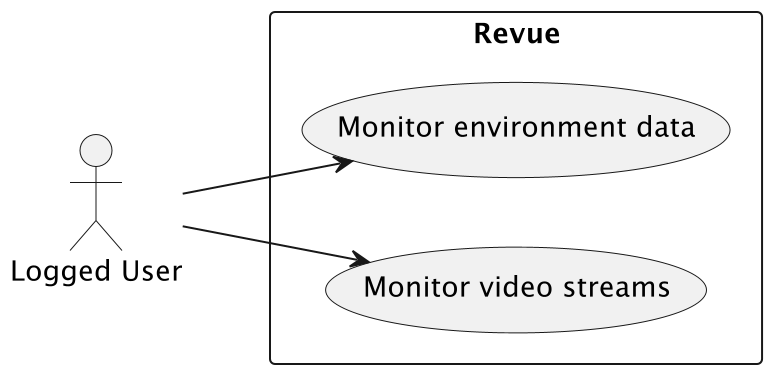
\includegraphics[scale=0.6]{img/simple-use-case}
        \caption{Simple Use Case}
        \label{fig:simple-use-case}
    \end{figure}

    A more complex scenario could involve both sensor and camera usages with the support of n intelligent feature to detect intrusion.
    %
    For example, the director of food wholesale could monitor the temperature of the warehouse and the presence of unauthorized people during the night.
    %
    In this case, the recognition part of the system is necessary to detect whenever an intrusion occurs.

    Moreover, supply chain monitoring can be done for who's needs to ensure that the temperature of
    the warehouse is always in the right range and be alerted whenever the temperature exceeds a certain range to detect or
    prevent problems.

    \begin{figure}
        \centering
        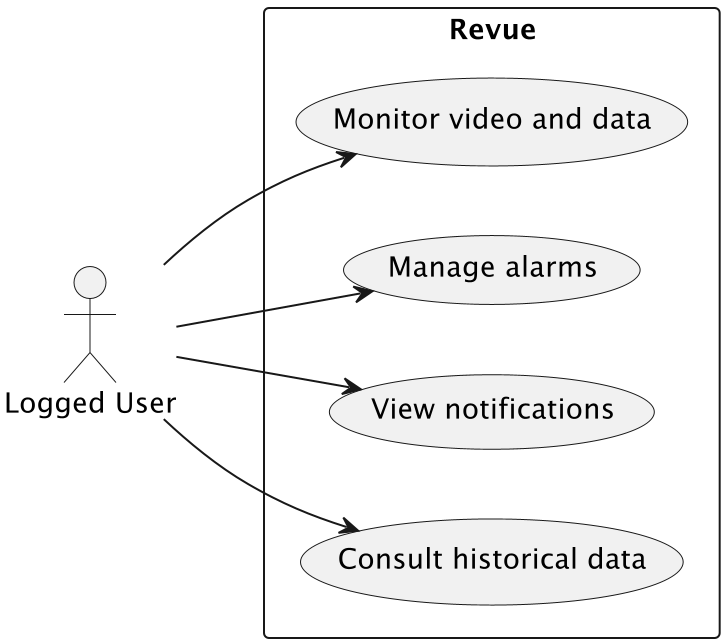
\includegraphics[scale=0.6]{img/advanced-use-case}
        \caption{Advanced Use Case}
        \label{fig:advanced-use-case}
    \end{figure}

    \subsection{Self-assessment policy}

    The project can be considered completed when \textbf{all} requirements are satisfied.

    In particular, non-functional requirements aim to grant a good general quality of the system.
    This will be achieved also using automated tests that will ensure, among other things, the quality of code production.

    \section{Requirements Analysis}

%Is there any implicit requirement hidden within this project's requirements?
%
%Is there any implicit hypothesis hidden within this project's requirements?
%
%Are there any non-functional requirements implied by this project's requirements?

%What model / paradigm / techonology is the best suited to face this project's requirements?
%
%What's the abstraction gap among the available models / paradigms / techonologies and the problem to be solved?

    Drawing up requirements, one relevant considered topic is the recognition feature.
    %
    This is supposed to be developed using Python and exploiting its main libraries for video processing and object recognition, to minimize the abstraction gap.

    Another important aspect is the handling of video streams.
    %
    In fact, to facilitate the development, an implicit requirement is necessary: the use of an ad hoc \textit{media server}.
    %
    This permits also improving the compatibility permitting to produce and consume using different protocols.

    Eventually, internal communications between devices and services need to be guaranteed.
    %
    This implicitly leads to the use of a message broker (\textit{Kafka}) which guarantees better scalability and at least one message delivery policy.


    \section{Design}

    \subsection{Ubiquitous Language}

    For the initial design phase, it's useful to define a common language that permits referring to the concepts with coherence and no ambiguity.
    This is a fundamental part of Domain Driven Design philosophy.

    In \cref{tab:ubiquitous-language} is shown the designed ubiquitous language, while in \cref{tab:synonyms} are reported the synonyms.

    \renewcommand{\arraystretch}{1.5}
    \begin{table}
        \centering
        \begin{tabularx}{0.7\textwidth}{ | c | >{\centering\arraybackslash}X | }
            \hline
            \textbf{Term} & \textbf{Meaning} \\
            \hline
            Camera & Device that generates a video stream and sends it to the other parts of the system \\
            \hline
            Sensor & Device capturing sensing data from an environment (e.g.\ temperature) \\
            \hline
            Device & Either a camera or a sensor \\
            \hline
            Video Stream & Stream of video data produced by a camera \\
            \hline
            Environment Data & Data produced by a sensor \\
            \hline
            User & User that can access the system \\
            \hline
            Detection & Recognition of an object in a video stream \\
            \hline
            Intrusion & Detection of an unauthorized object \\
            \hline
            Exceeding & Environment value exceeding user defined ranges \\
            \hline
            Anomaly & Either an intrusion or an exceeding \\
            \hline
            Security Rule & Rule defined by the supervisor to trigger anomalies in a defined range of time \\
            \hline
            Notification & An alert sent to the user to inform that an anomaly has been triggered. \\
            \hline
        \end{tabularx}
        \caption{Ubiquitous Language}
        \label{tab:ubiquitous-language}
    \end{table}

    \renewcommand{\arraystretch}{1.8}
    \begin{table}
        \centering
        \begin{tabularx}{0.6\textwidth}{ | >{\centering\arraybackslash}X | >{\centering\arraybackslash}X | }
            \hline
            \textbf{Term} & \textbf{Synonyms} \\
            \hline
            Camera & Video camera \\
            \hline
            Video Stream & Video, Transmission \\
            \hline
            Environment Data & Data, Sensing Data \\
            \hline
            User & Supervisor, Admin \\
            \hline
            Security Rule & Rule \\
            \hline
        \end{tabularx}
        \caption{Synonyms}
        \label{tab:synonyms}
    \end{table}

    \subsection{Architecture}

    The overall system is designed with microservices architecture.
    %
    This choice helped us to increase modularity, scalability, reliability and fault tolerance.
    %
    The system is composed of the following microservices:

    \begin{itemize}
        \item \textbf{Authentication Service}: responsible for the authentication and access control.
        \item \textbf{Monitoring Service}: responsible for managing devices and environment data.
        \item \textbf{Recognition Service}: responsible for the recognition of objects in the video streams.
        \item \textbf{Alarm Service}: responsible for the management of the security rules and anomalies.
        \item \textbf{Notification Service}: responsible for sending notifications to the user.
        \item \textbf{Log Service}: responsible for the persistent saving of data.
    \end{itemize}

    Each microservice consists of
    \begin{enumerate*}
        \item Web server exposing REST APIs
        \item Database to store its data (except for the \textbf{Recognition Service})
    \end{enumerate*}
    (\cref{fig:microservice}).

    \begin{figure}
        \centering
        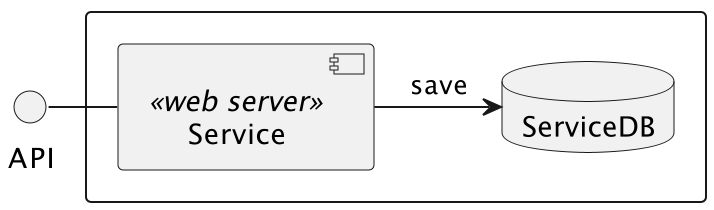
\includegraphics[scale=0.6]{img/microservice}
        \caption{Microservice components}
        \label{fig:microservice}
    \end{figure}

    Moreover, other components are necessary to make the system work:

    \begin{itemize}
        \item \textbf{Frontend}: provides to the user the web interface to interact with the system.
        \item \textbf{Sensors}: captures the environment data and send them to the rest of the system.
        \item \textbf{Cameras}: captures the video streams and send them to the rest of the system.
        \item \textbf{Media Server}: used to consume the produced video streams and make them available using different protocols.
        \item \textbf{Broker}: used to manage some internal communications.
    \end{itemize}

    In \cref{fig:architecture} is presented the whole architecture diagram.

    \begin{figure}
        \centering
        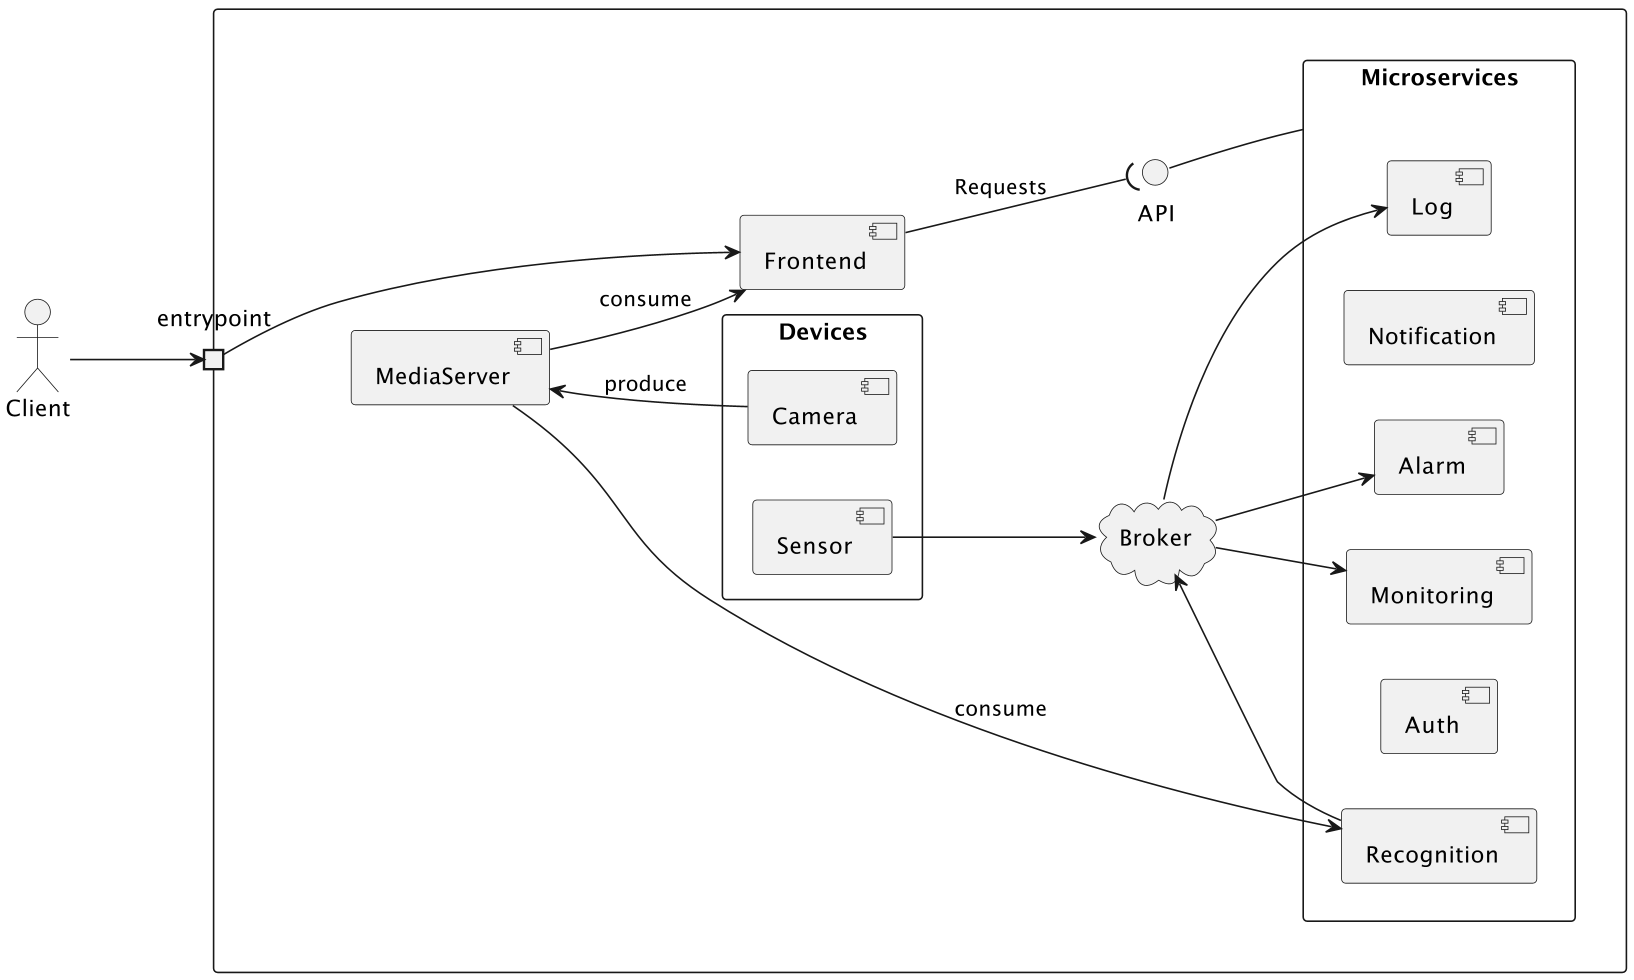
\includegraphics[scale=0.51]{img/architecture}
        \caption{Revue Architecture}
        \label{fig:architecture}
    \end{figure}


    \subsection{Structure}

%    Which entities need to be modelled to solve the problem?
%%
%    (UML Class diagram)
%
%    How should entities be modularised?
%%
%    (UML Component / Package / Deployment Diagrams)

    For the design phase, Domain Driven Design (DDD) and Hexagonal Architecture (HA) have been adopted.
    %
    Actually, the adherence to DDD and HA can be considered a little bit rough (for example, because of the lack of an ad hoc presentation layer) and it will be improved in the future.

    To briefly specify the layers' dependencies:
    \begin{itemize}
        \item \textbf{Domain} layer cannot depend on any other layer.
        \item \textbf{Application} layer (which contains business logic) can depend only on Domain layer.
        \item \textbf{Storage} layer depends on the layers above.
        It is the outer layer since it contains platform-dependent implementation.
    \end{itemize}

    Each microservice has the same structure in terms of classes and packages.
    %
    Furthermore, it is responsible for a specific subset of domain entities.

    In \cref{fig:general-structure}, is represented the general packages/classes structure.

    To not replicate all the code in the microservices, a shared module called \textbf{domain} has been created.
    This is possible due to the fact most of the microservices share the same platform (Node.js).
    The exception is the \textbf{Recognition} service, which is implemented in Python, and it required a reimplementation of some domain entities.

    \begin{figure}
        \centering
        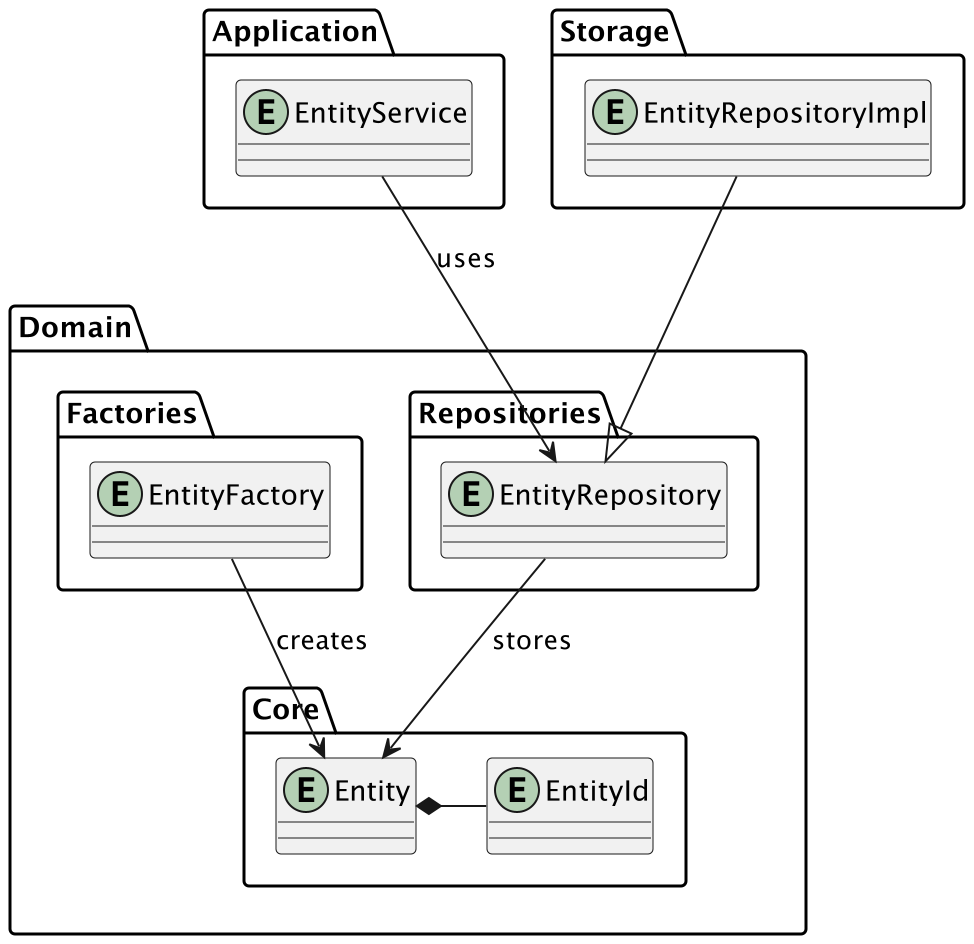
\includegraphics[scale=0.55]{img/general-structure}
        \caption{General structure of microservice}
        \label{fig:general-structure}
    \end{figure}

    \subsection{Behaviour}

    \subsubsection{Monitoring Service}

    \textbf{Monitoring} is the microservice in charge of retrieving environment data from the \textbf{Broker} produced by the sensors,
    and to provide them to the user through the \textbf{Frontend}.
    It allows also adding, delete or modify a device configuration, and it is responsible for the management of the devices.

    \subsubsection{Recognition Service}

    \textbf{Recognition} microservice performs in loop object recognition on cameras' video streams.
    Initially, it gets the intrusion rules from the \textbf{Alarm} service.
    Then, it connects to the \textbf{Media Server} to consume the video streams.
    When a predefined object is recognised, it sends it to the \textbf{Alarm} service.

    Periodically, it checks if the intrusion rules, or their validity, have changed.

    Foreach camera subject to an active rule, it spawns a new process to perform the recognition.
    When there is no more active rule for a camera, the process terminates.

    An activity diagram is shown in \cref{fig:recognition-activity}.

    \begin{figure}
        \centering
        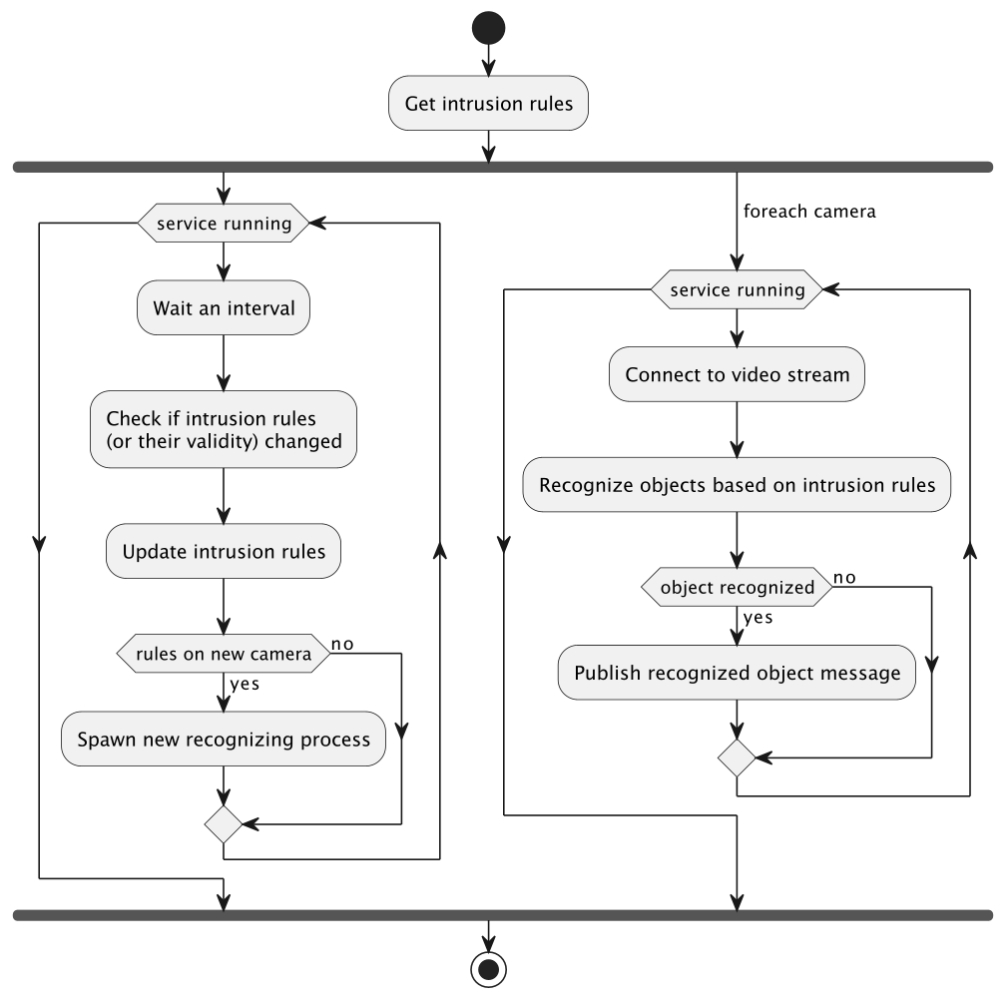
\includegraphics[scale=0.6]{img/recognition-activity}
        \caption{Recognition service activity diagram}
        \label{fig:recognition-activity}
    \end{figure}


    \subsubsection{Alarm Service}

    \textbf{Alarm} microservice is responsible for the anomalies' detection.
    It is able to check the data coming from the sensors or the recognised objects on cameras' streams.
    The service needs to check active rules for active devices.
    It is able to create an anomaly, store it, and notify the \textbf{Notification} service if the data is not compliant with the rules (\cref{fig:alarm-activity}).

    Moreover, this service is in charge of the security rules management, allowing the user to modify their configuration.

    \begin{figure}
        \centering
        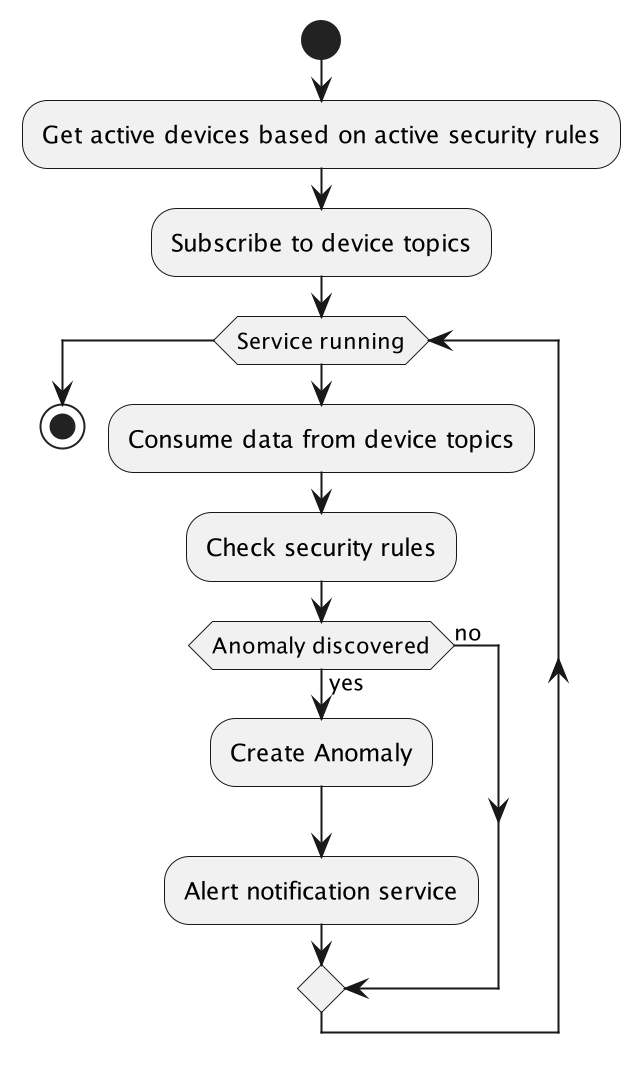
\includegraphics[scale=0.24]{img/alarm-activity}
        \caption{Alarm service activity diagram}
        \label{fig:alarm-activity}
    \end{figure}

    \subsubsection{Notification Service}
    This microservice is responsible to notify the user in case of anomalies.
    When the \textbf{Alarm} service detects an intrusion or an exceeding, it sends a message to the \textbf{Notification}
    service that will notify the user through an email or an SMS\@.

    If the user is logged in through \textbf{Frontend}, the notification will be sent in real-time using sockets.

    \subsubsection{Log Service}
    Microservice responsible for the storage of the environment data produced by sensors.
    It is simply listening to the \textbf{Broker} and storing the published data in the database.
    It also allows the user to consult the historical data of the environment.

    \subsubsection{Devices}

    Devices, both cameras and sensors, are responsible for producing data and sending them to the \textbf{Broker}.
    Once initialised, they start to produce data, in particular:
    \begin{itemize}
        \item Sensors publish environment data on a topic.
        \item Cameras publish video streams with RTSP protocol to the \textbf{Media Server}.
    \end{itemize}

    Actually, both devices are simulated.
    Sensor nodes produce random data, while the camera nodes stream a local video file.


    \begin{figure}
        \centering
        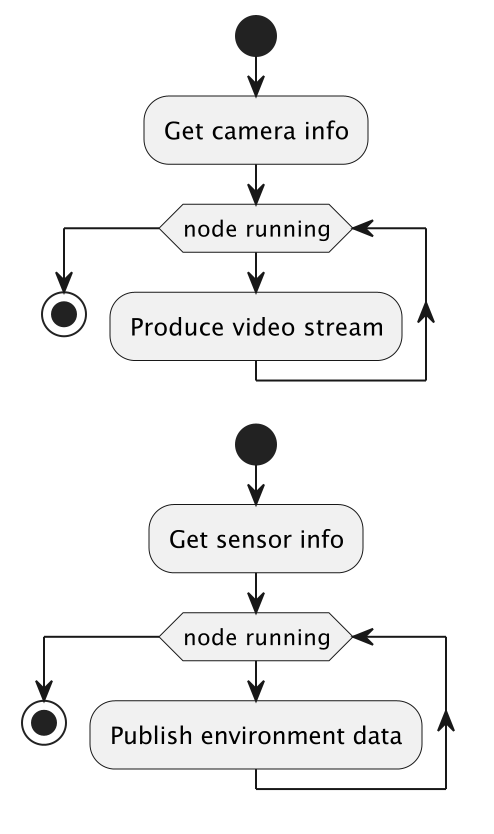
\includegraphics[scale=0.6]{img/device-activity}
        \caption{Device activity diagram}
        \label{fig:device-activity}
    \end{figure}


    \subsection{Interaction}

    \subsubsection{Authentication}
    \begin{figure}
        \centering
        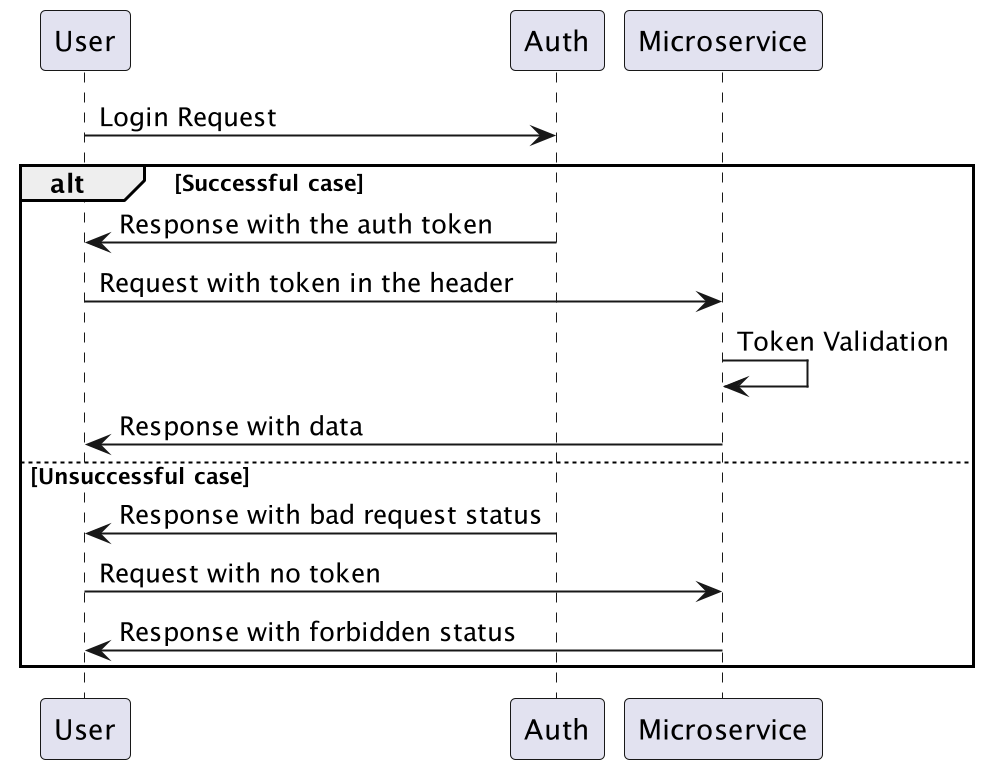
\includegraphics[scale=0.3]{img/auth-service-sequence}
        \caption{Auth service sequence diagram}
        \label{fig:auth-service-sequence}
    \end{figure}

    The \textbf{Auth} service is responsible for the authentication process (\cref{fig:auth-service-sequence}).

    When a login request is performed, the \textbf{Auth} service checks the credentials and returns an access token if the authentication is successful.
    Whenever a request to another service is performed, the access token is sent in the header.
    Every service contains a validation middleware through which the token is checked.

    This process has been implemented using the Json Web Token (JWT) and sharing the secret key between federated services.

    \subsection{Video Stream}
    \begin{figure}
        \centering
        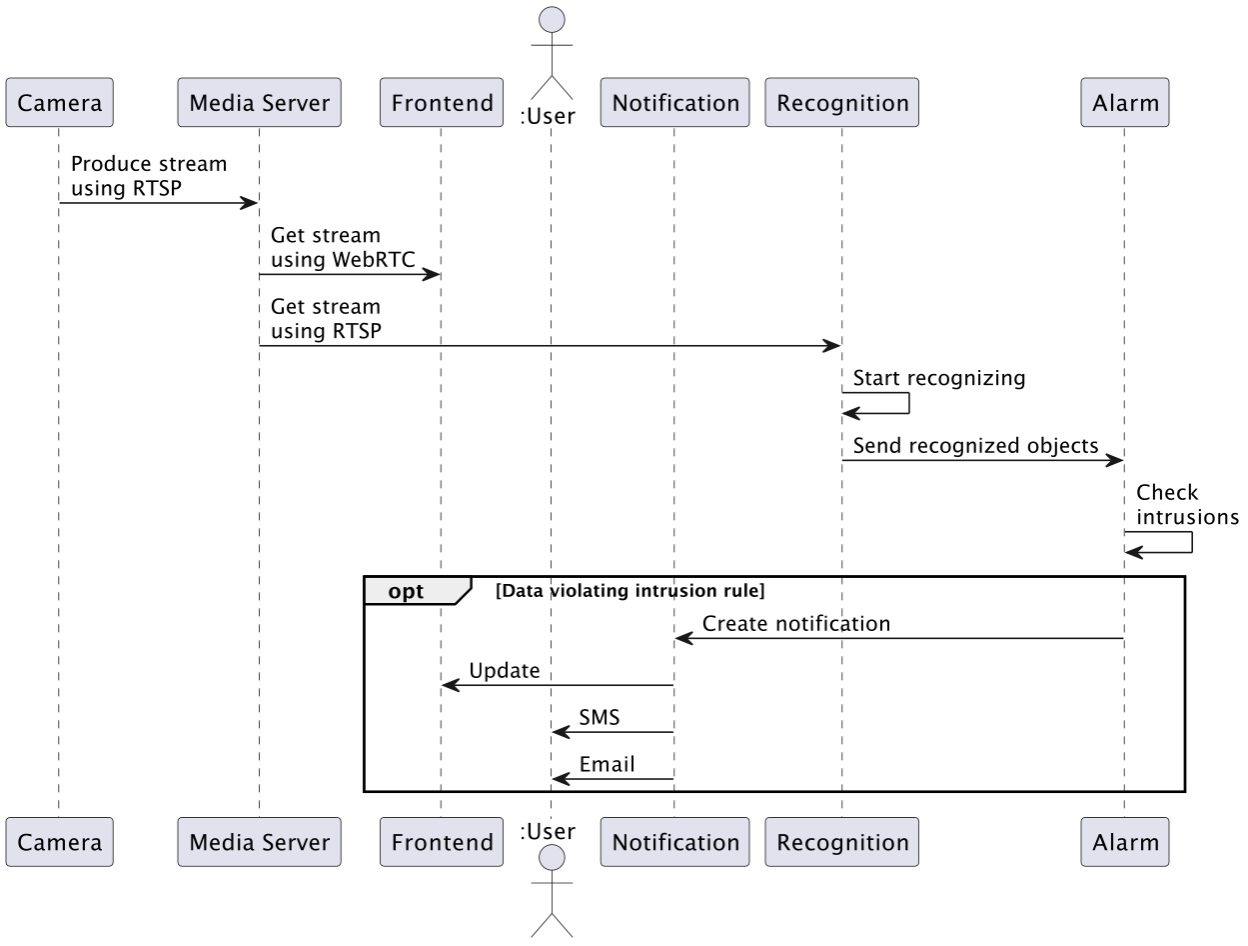
\includegraphics[scale=0.5]{img/video-stream-sequence}
        \caption{Video stream sequence diagram}
        \label{fig:video-stream-sequence}
    \end{figure}

    The handling of video stream involves a set of components as shown in \cref{fig:video-stream-sequence}.

    First of all, the camera sends the video stream to the \textbf{Media Server} using RTSP protocol.
    Then, the \textbf{Media Server} is responsible for making the stream available to whoever wants to consume it.

    In this case, the  \textbf{Recognition} service consumes the stream using RTSP protocol, while the \textbf{Frontend} consumes it using WebRTC protocol.

    \textbf{Recognition} service starts the image recognition process on the stream and sends the recognised objects to the \textbf{Alarm} service.
    The latter, in case of an intrusion (\cref{tab:ubiquitous-language}), will alert the  \textbf{Notification} service to notify the user.

    \subsection{Sensor Data Stream}
    \begin{figure}
        \centering
        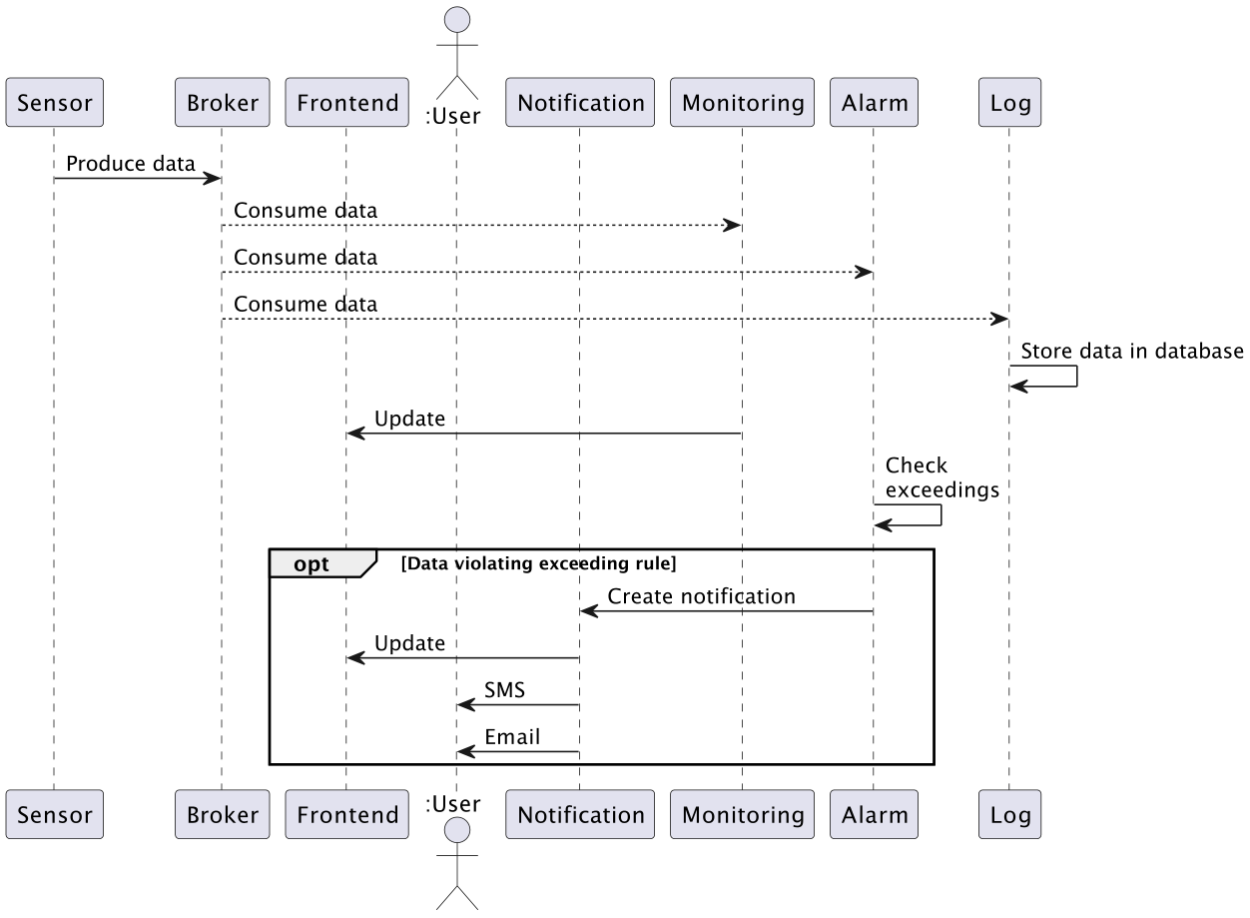
\includegraphics[scale=0.5]{img/sensor-data-sequence}
        \caption{Sensor data sequence diagram}
        \label{fig:sensor-data-sequence}
    \end{figure}

    In the sensor data stream scenario (\cref{fig:sensor-data-sequence}), what happens is analogous to the video stream scenario.

    Sensors continuously produce data, publishing them to the \textbf{Broker}.
    In the standard case, three services will consume the data:

    \begin{itemize}
        \item \textbf{Monitoring} service, to make the data available to the user through the \textbf{Frontend}.
        \item \textbf{Alarm} service, to check the data against the security rules.
        \item \textbf{Log} service, to store the data persistently.
    \end{itemize}

    In case of an exceeding (\cref{tab:ubiquitous-language}), the same notification process as the video stream scenario will be triggered.

    \section{Implementation Details}

    \subsection{Kafka}

    \href{https://kafka.apache.org}{Apache Kafka} is the technology chosen to handle intra-system real-time communications.

    In particular, \href{https://kafka.js.org}{KafkaJS} and \href{https://kafka-python.readthedocs.io/en/master/}{kafka-python} clients
    have been used respectively for the \href{https://nodejs.org/en}{Node.js} and \href{https://flask.palletsprojects.com/en/3.0.x/}{Flask} services.

    Kafka is an open-source distributed event streaming platform capable of handling plenty of events per second.

    In the following, is reported the code for producing (\Cref{lst:kafka-producer}) and consuming (\Cref{lst:kafka-consumer}) messages using KafkaJS.

    \lstinputlisting[
        language=TypeScript,
        caption={Producing using KafkaJS},
        label={lst:kafka-producer},
    ]{code/producer.ts}

    \lstinputlisting[
        language=TypeScript,
        caption={Consuming using KafkaJS},
        label={lst:kafka-consumer},
    ]{code/consumer.ts}

    \subsection{Sockets}
    \href{https://socket.io/}{Socket IO} is a library that enables real-time, bidirectional and event-based communication between the browser and the server.
    It has been exploited to implement the real-time communication between the user and the system, in particular for pushing notifications or sending the environment data to the user.
    A security layer has been added to socket servers to ensure secure connections.
    Also for this feature, the JWT token generated when the user logs in has been used.

    \lstinputlisting[
        language=TypeScript,
        caption={Socket Server middleware},
        label={lst:socket-middleware},
    ]{code/sockets.ts}

    \subsection{Object Recognition with YOLO}
    You only look once (\href{https://pjreddie.com/darknet/yolo}{YOLO}) is a state-of-the-art, efficient real-time object detection algorithm.
    %
    YOLO is able to recognise classes of objects and its position in the video.

    This algorithm is used within the \textbf{Recognition} service to perform object recognition on video stream produced by the cameras, according to active security rules.

    In \Cref{lst:object-recognition} is reported the responsible code for this task.
    \lstinputlisting[
        language=Python,
        label={lst:object-recognition},
        caption={Python class performing object recognition with YOLO},
    ]{code/Recognizer.py}


    \subsection{Media Server}
    \href{https://github.com/bluenviron/mediamtx}{MediaMTX} has been used to allow the system to support more than one protocol without implementing a single procedure for each of them.
    All the cameras connect to the media server, it can be used to retrieve the video streams using different protocols.

    In this case, RTSP protocol is used from cameras to produce video streams and from \textbf{Recognition} to consume video streams.
    Instead, WebRTC protocol is used to consume video streams from the \textbf{Frontend}.

    \subsection{WebRTC}
    To simulate the camera streams, the \href{https://webrtc.org/}{WebRTC} protocol takes place.
    It has been selected for its ability to stream video and audio in real-time with simplicity.
    It does not require any plugin or software installation, it is supported by all the major browsers, and it is open-source.
    Developed by Google, it implements the Google Congestion Control \href{https://www.researchgate.net/publication/316684665_Congestion_Control_for_Real-Time_Communication}{(GCC)} algorithm that allows to stream video and audio in real-time with a low latency.

    \subsection{Single Sign-On}
    \href{https://en.wikipedia.org/wiki/Single_sign-on}{The Single Sign-On (SSO)} has been implemented to allow the user to access the system with a single set of credentials.
    The \textbf{Auth} service is responsible for the authentication of the user and the generation of the \href{https://jwt.io/}{Json Web Token} (JWT) token that will be used to authenticate the user in the other services.
    The generated token can be validated from each microservice to ensure that the user is authenticated.
    Following this approach, in case of failure of the authentication service, the user can still access the system until its token validity expires.
    Moreover, the single point of failure is avoided.
    This process has been implemented through the use of JWT and sharing the secret key between federated services.

    \lstinputlisting[
        language=TypeScript,
        caption={Middleware for the microservices},
        label={lst:microservice-middleware},
    ]{code/sso.ts}

    \section{Self-assessment / Validation}

    \subsection{Quality Assurance}\label{subsec:quality-assurance}

    Two main tools have been used to ensure the quality of the code produced:

    \begin{itemize}
        \item \href{https://prettier.io/}{Prettier} is a code formatter that supports many languages.
        It enforces a consistent style by parsing code and re-writing it according to the configuration rules.
        \item \href{https://eslint.org/}{ESLint} is a tool that statically analyses code to find suboptimal patterns and errors.
    \end{itemize}

    Both tools have been integrated into the Continuous Integration pipeline (\cref{subsec:continuous-integration}) to keep the high-quality code production.

    \subsection{Architectural Testing}\label{subsec:architecture-testing}

    In order to ensure that layers' dependencies are respected, \href{https://github.com/sverweij/dependency-cruiser}{Dependency Cruiser} framework has been exploited.

    Essentially, the configured rules check that:

    \begin{itemize}
        \item \textbf{Domain} layer does not access to any other layer.
        \item \textbf{Application} layer can access only the Domain layer.
        \item \textbf{Presentation} layer can access only Domain and Application layers.
    \end{itemize}

    \subsection{API Testing}\label{subsec:api-testing}

    API testing has been performed using \href{https://vitest.dev/}{Vitest} framework.

    To be able to execute the tests, the database has been mocked using \href{https://github.com/nodkz/mongodb-memory-server}{MongoDB Memory Server}.

    In \Cref{lst:api-test} is reported a simplified example of an API test.

    \lstinputlisting[
        language=TypeScript,
        label={lst:api-test},
        caption={API testing example},
    ]{code/api-test.ts}


    \subsection{Fault Tolerance Testing}\label{subsec:fault-tolerance-testing}

    Since reliability is an important non-functional requirement (requirement \ref{itm:non-func-1}),
    a specific script has been set up to test the system behaviour in case of faults.

    In \Cref{lst:fault-tolerance-test} is reported the main part of the script used to
    \begin{enumerate*}
        \item Tearing up the system
        \item Tearing down some running services
        \item Executing fault tolerance tests.
    \end{enumerate*}

    Nevertheless, script and tests could be improved by adding new different fault scenarios.

    \lstinputlisting[
        language=bash,
        label={lst:fault-tolerance-test},
        caption={API testing example},
    ]{code/fault-tolerance-tests.sh}

    \subsection{Continuous Integration}\label{subsec:continuous-integration}

    Each test previously described in this section has been integrated into the Continuous Integration pipeline.

    \section{Deployment}

    \subsection{Prerequisites}

    \begin{itemize}
        \item Docker
    \end{itemize}

    \subsection{Starting the system}

    To deploy the whole system:
    \begin{enumerate}
        \item Clone the project from \href{https://github.com/Mala1180/revue/}{Revue}.
        \item Navigate to the project root.
        \item Run the \textit{deploy.sh} script.
    \end{enumerate}

    Once the system is up and running, the web interface entrypoint is available at \href{http://localhost:8080}{http://localhost:8080}.
    The credentials of the example user are:
    \begin{itemize}
        \item Username: \texttt{user}
        \item Password: \texttt{user}
    \end{itemize}

    To tear down the system, run the \textit{undeploy.sh} script.

    In addiction to already cited entities, is present a \href{https://zookeeper.apache.org}{Zookeeper} container that is necessary for Kafka to work properly.

    To simulate running devices, two containers for each device are deployed.
    Note that if more devices are needed, it is necessary to manually add more containers to the docker-compose file in devices' modules (\textbf{sensor} and \textbf{camera}).
    It is also necessary, when adding new devices through the web interface, inserting the same device code used in the docker-compose file.

    \subsection{Starting sub-parts of the system}

    Other scripts are available to start the system differently, in order to:

    \begin{itemize}
        \item Deploy only some services with their databases, using the \textit{compose-service.sh} script.
        \item Deploy only databases, using the \textit{compose-db.sh} script.
    \end{itemize}

    Usage examples:

    \begin{itemize}
        \item \verb|./scripts/compose-service.sh --up auth monitoring frontend log|
        \item \verb|./scripts/compose-db.sh --up auth monitoring frontend log|
    \end{itemize}

    NB: Scripts have to be launched from the root of the project.

    \subsection{Configurations}
    In the root of the project, there is a \textit{.env} that contains the environment variables needed to correctly configure the system.
    Without modifying the \textit{.env} file, the services will be exposed on different ports according to \cref{tab:services-binding-ports}.

    \begin{table}
        \centering
        \begin{tabularx}{0.7\textwidth}{ | c | >{\centering\arraybackslash}X | >{\centering\arraybackslash}X | }
            \hline
            \textbf{Service name} & \textbf{Service Port} & \textbf{Database Port} \\
            \hline
            frontend & 8080 & ---\\
            \hline
            auth & 4000 & 27017 \\
            \hline
            monitoring & 4001 & 27018 \\
            \hline
            alarm & 4002 & 27019 \\
            \hline
            log & 4003 & 27020 \\
            \hline
            notification & 4004 & 27021 \\
            \hline
            recognition & 4005 & --- \\
            \hline
            media-server & 8554 rtsp & --- \\
            \hline
            kafka & 9092 & --- \\
            \hline
            zookeper & 2181 &  --- \\
            \hline
        \end{tabularx}
        \caption{Services binding ports}
        \label{tab:services-binding-ports}
    \end{table}

    \section{Usage Examples}

    For every usage, the system requires a login for security reasons.

    \begin{figure}
        \centering
        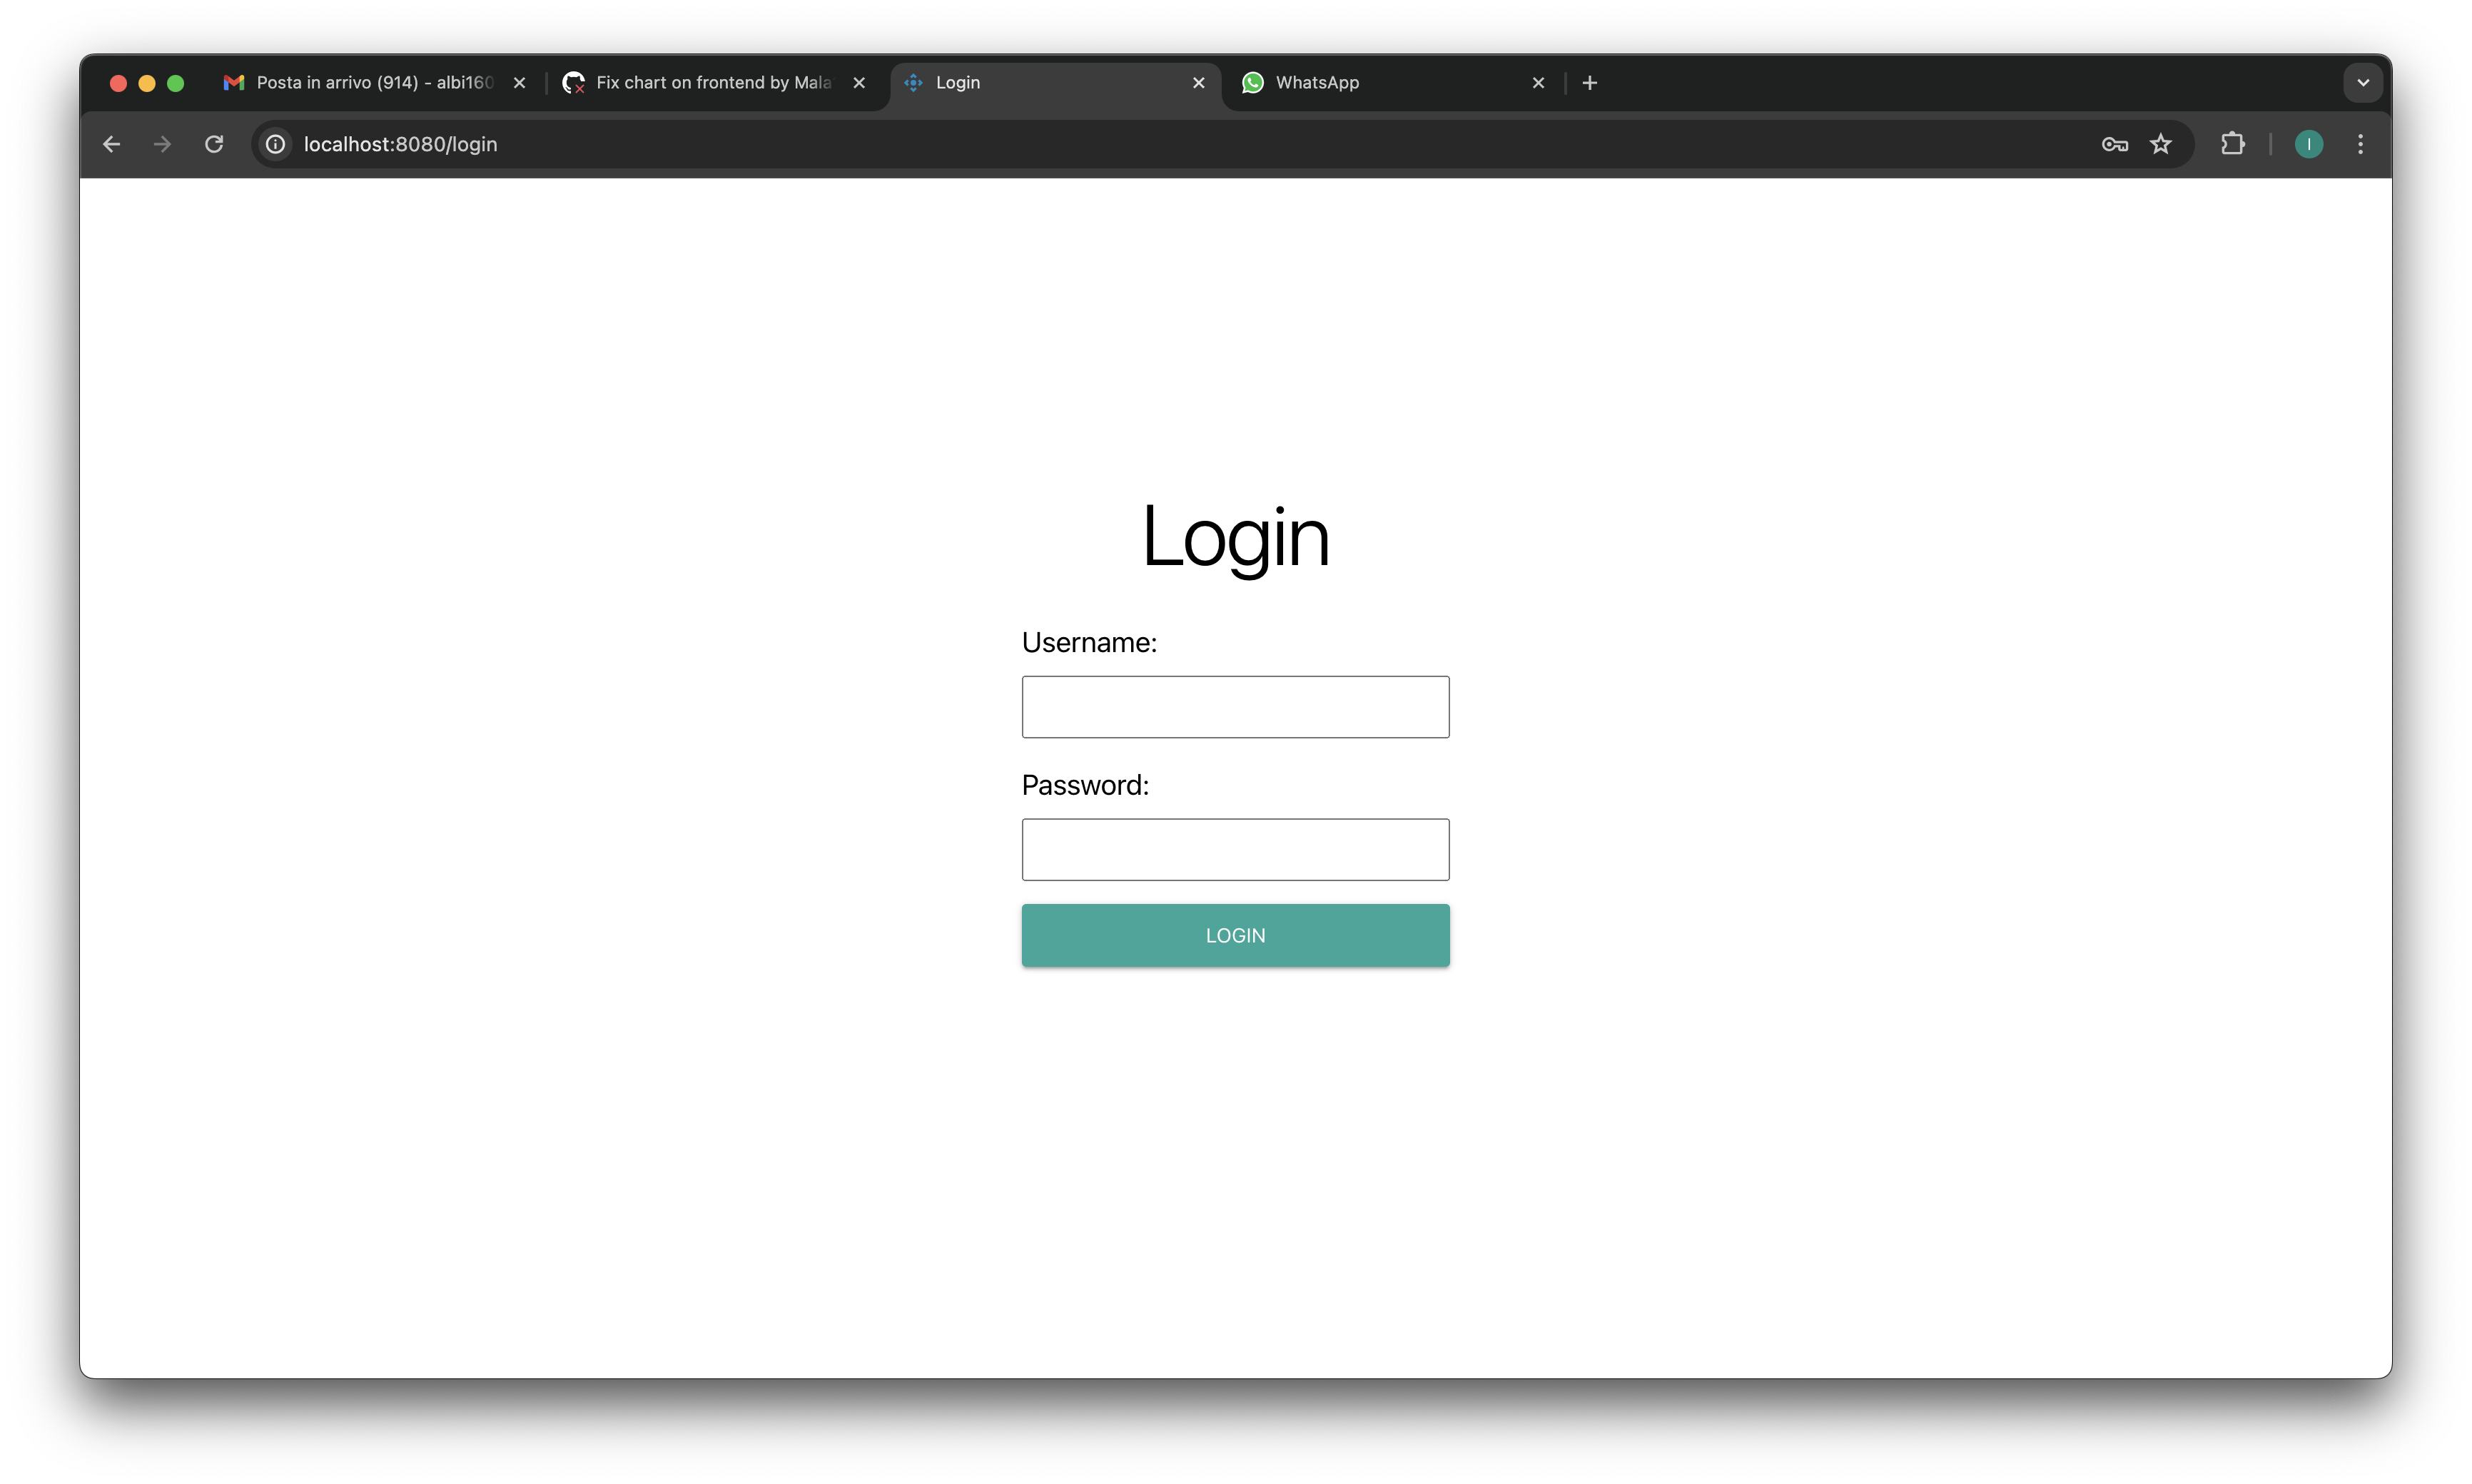
\includegraphics[scale=0.25]{img/usage/login_view}
        \caption{Login view}
        \label{fig:login-view}
    \end{figure}

    In the simplest scenario, the user can see the section designated for sensor environment data or the camera video streams consultation.

    \begin{figure}
        \centering
        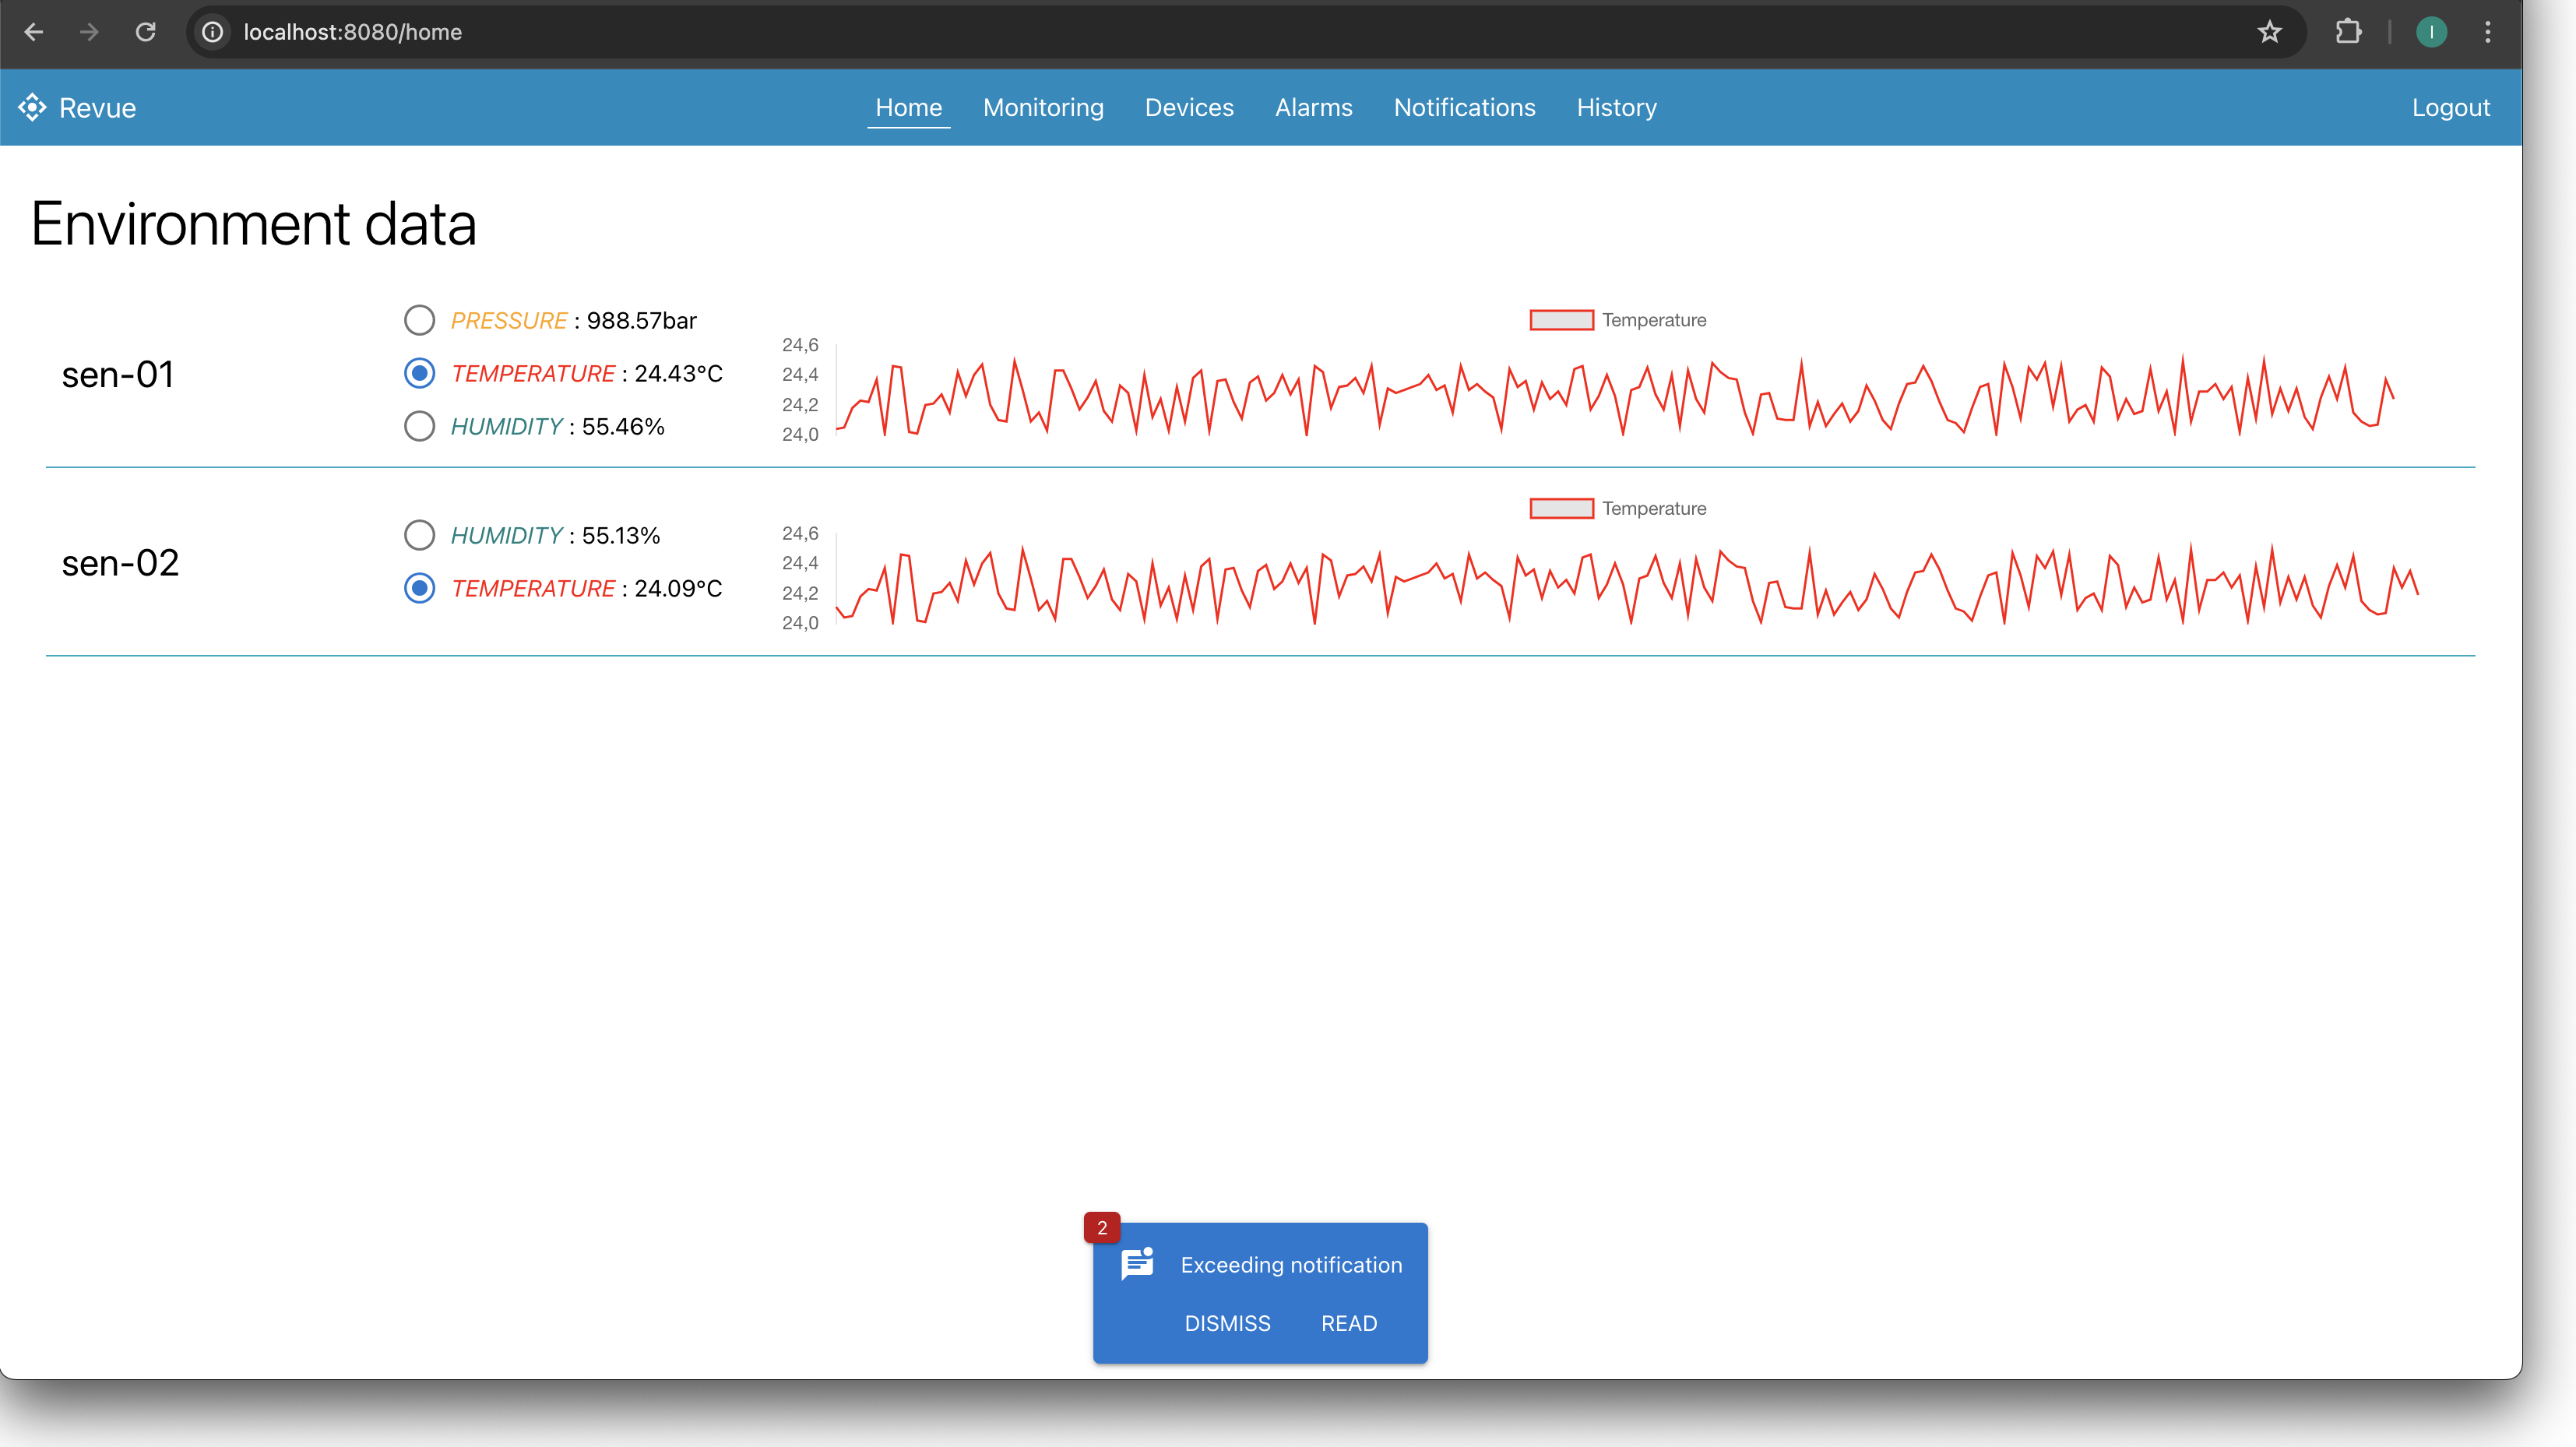
\includegraphics[scale=0.25]{img/usage/home_view}
        \caption{Home view}
        \label{fig:home-view}
    \end{figure}
    \begin{figure}
        \centering
        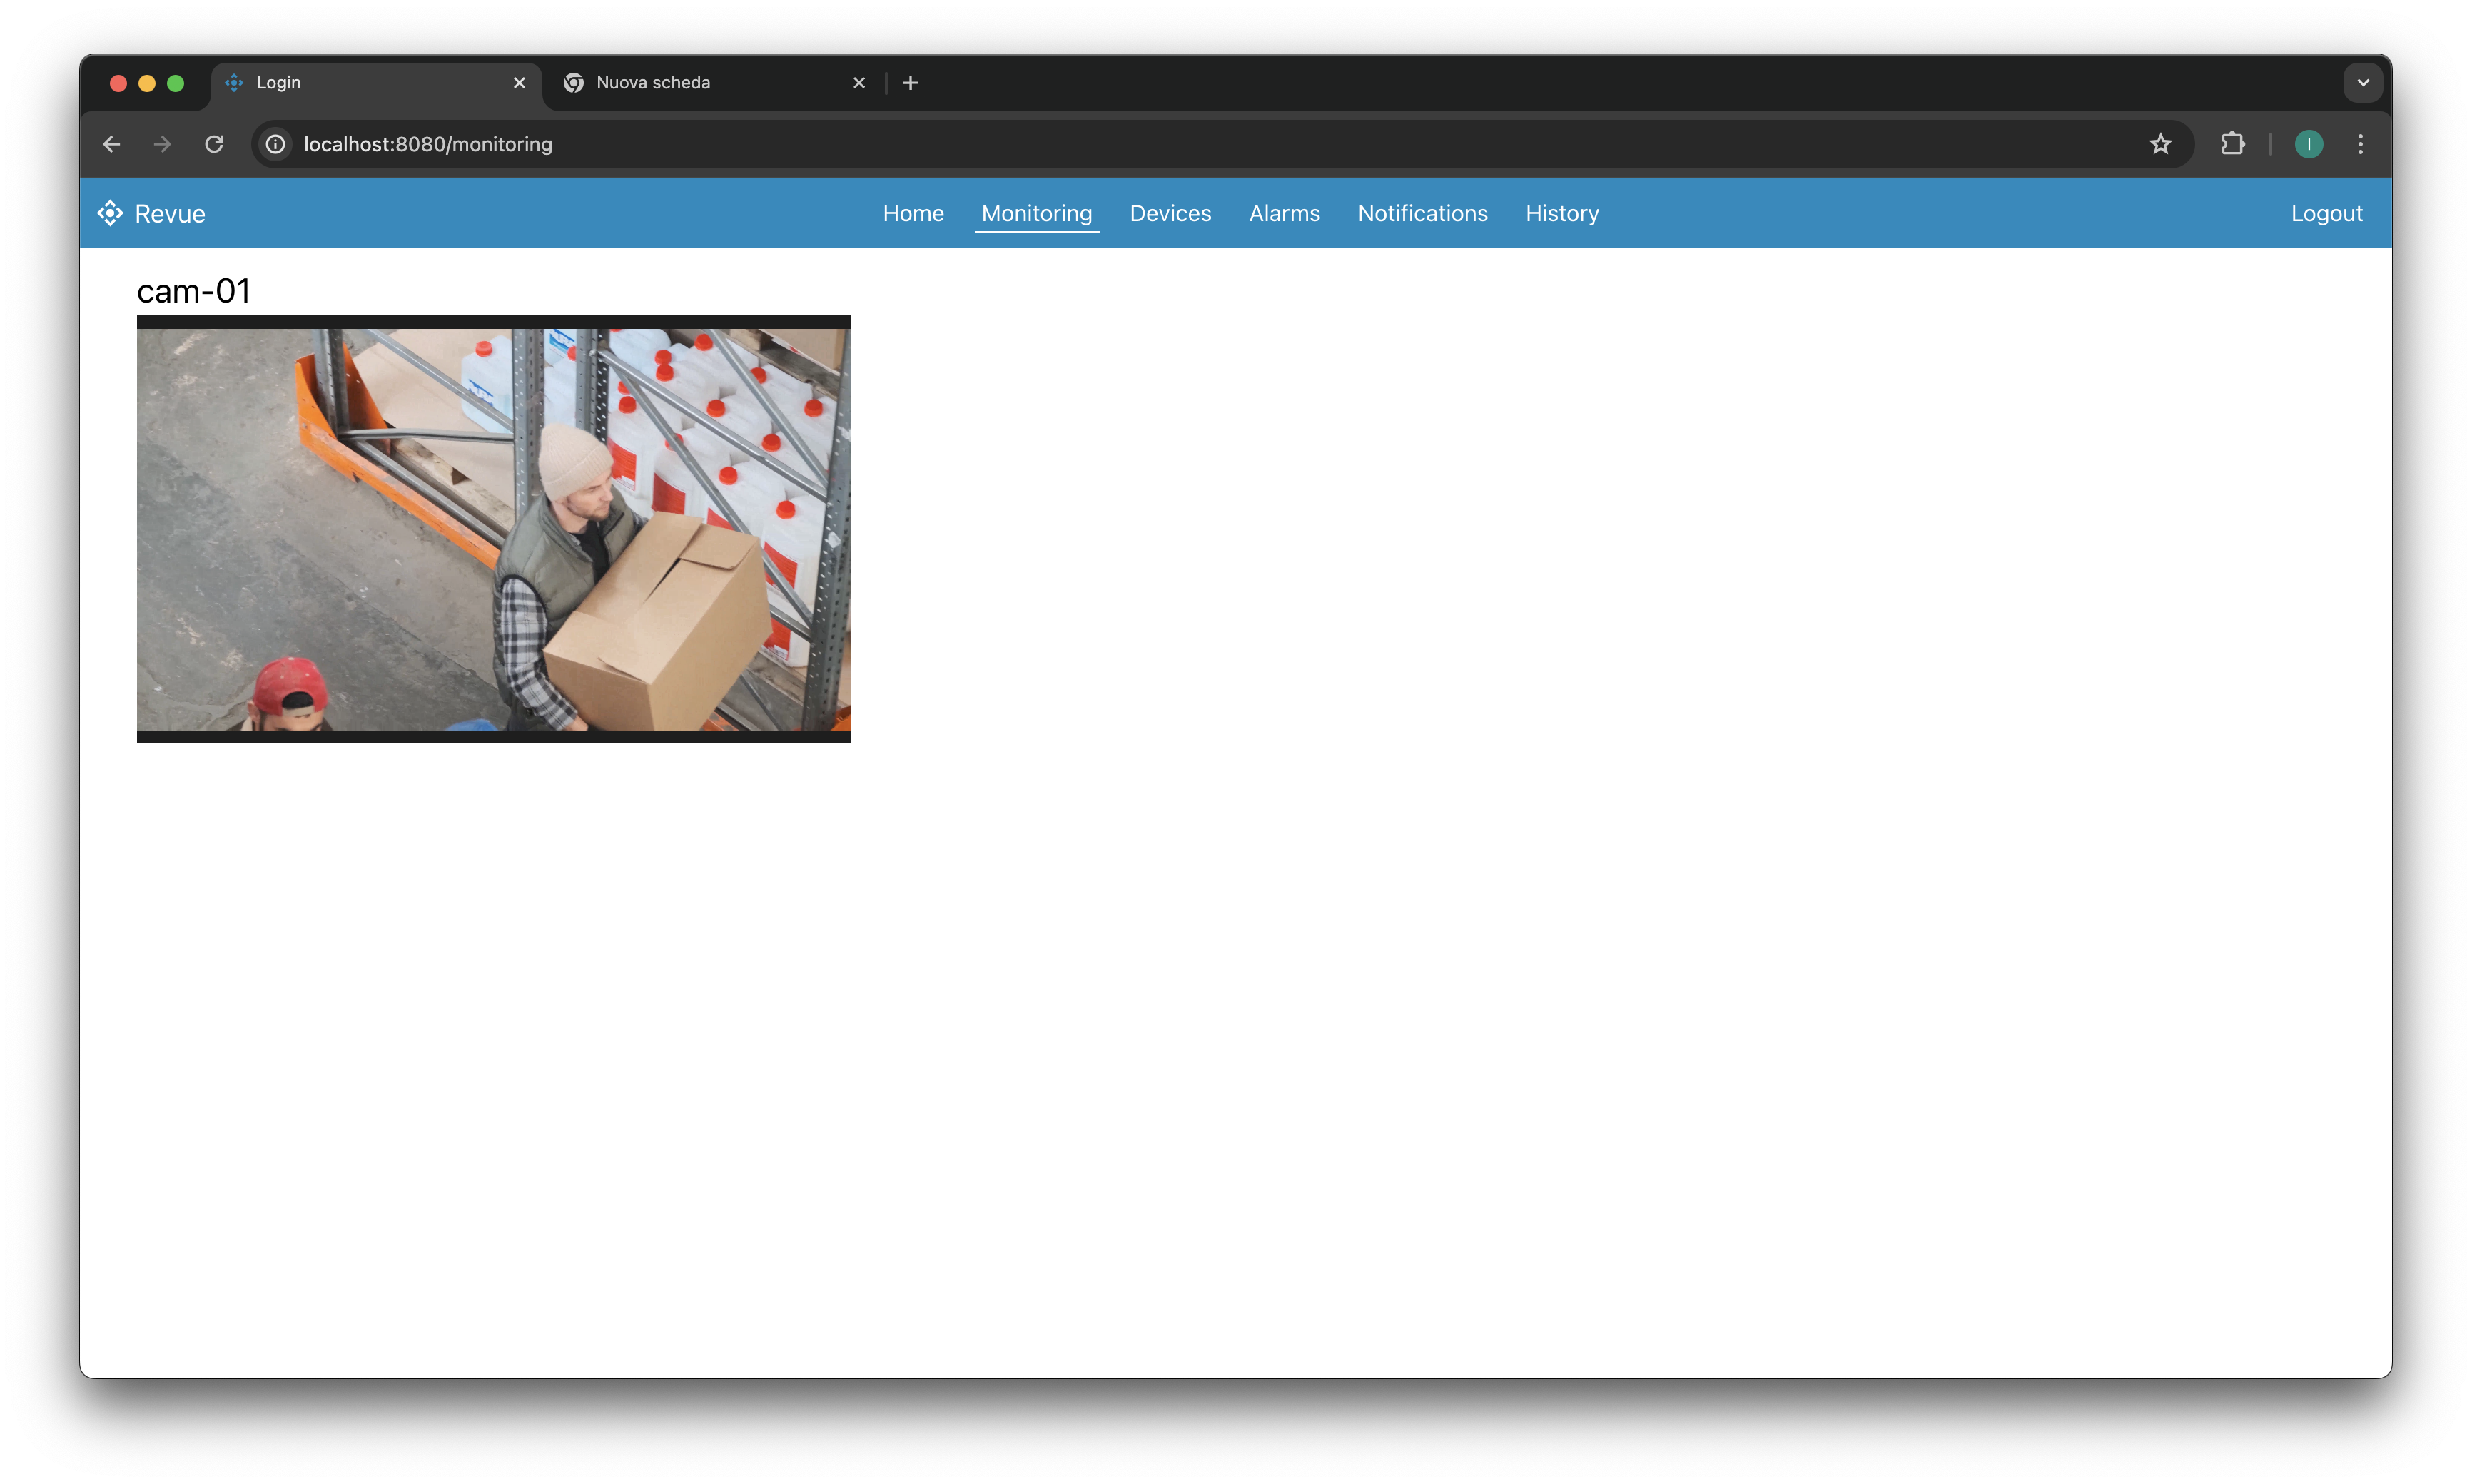
\includegraphics[scale=0.25]{img/usage/camera_view}
        \caption{Monitoring view}
        \label{fig:monitoring-view}
    \end{figure}


    In the more complex scenario, the user can add security rules to detect exceeding values or unauthorized objects in the video streams.

    When adding a new intrusion rule, the user can choose the object class to detect, the camera, and the time slot on which the rule will be active.

    Instead, when adding a new exceeding rule, the user specifies the range value (for a specific measure), the target sensor and the time slot validity.

    \begin{figure}
        \centering
        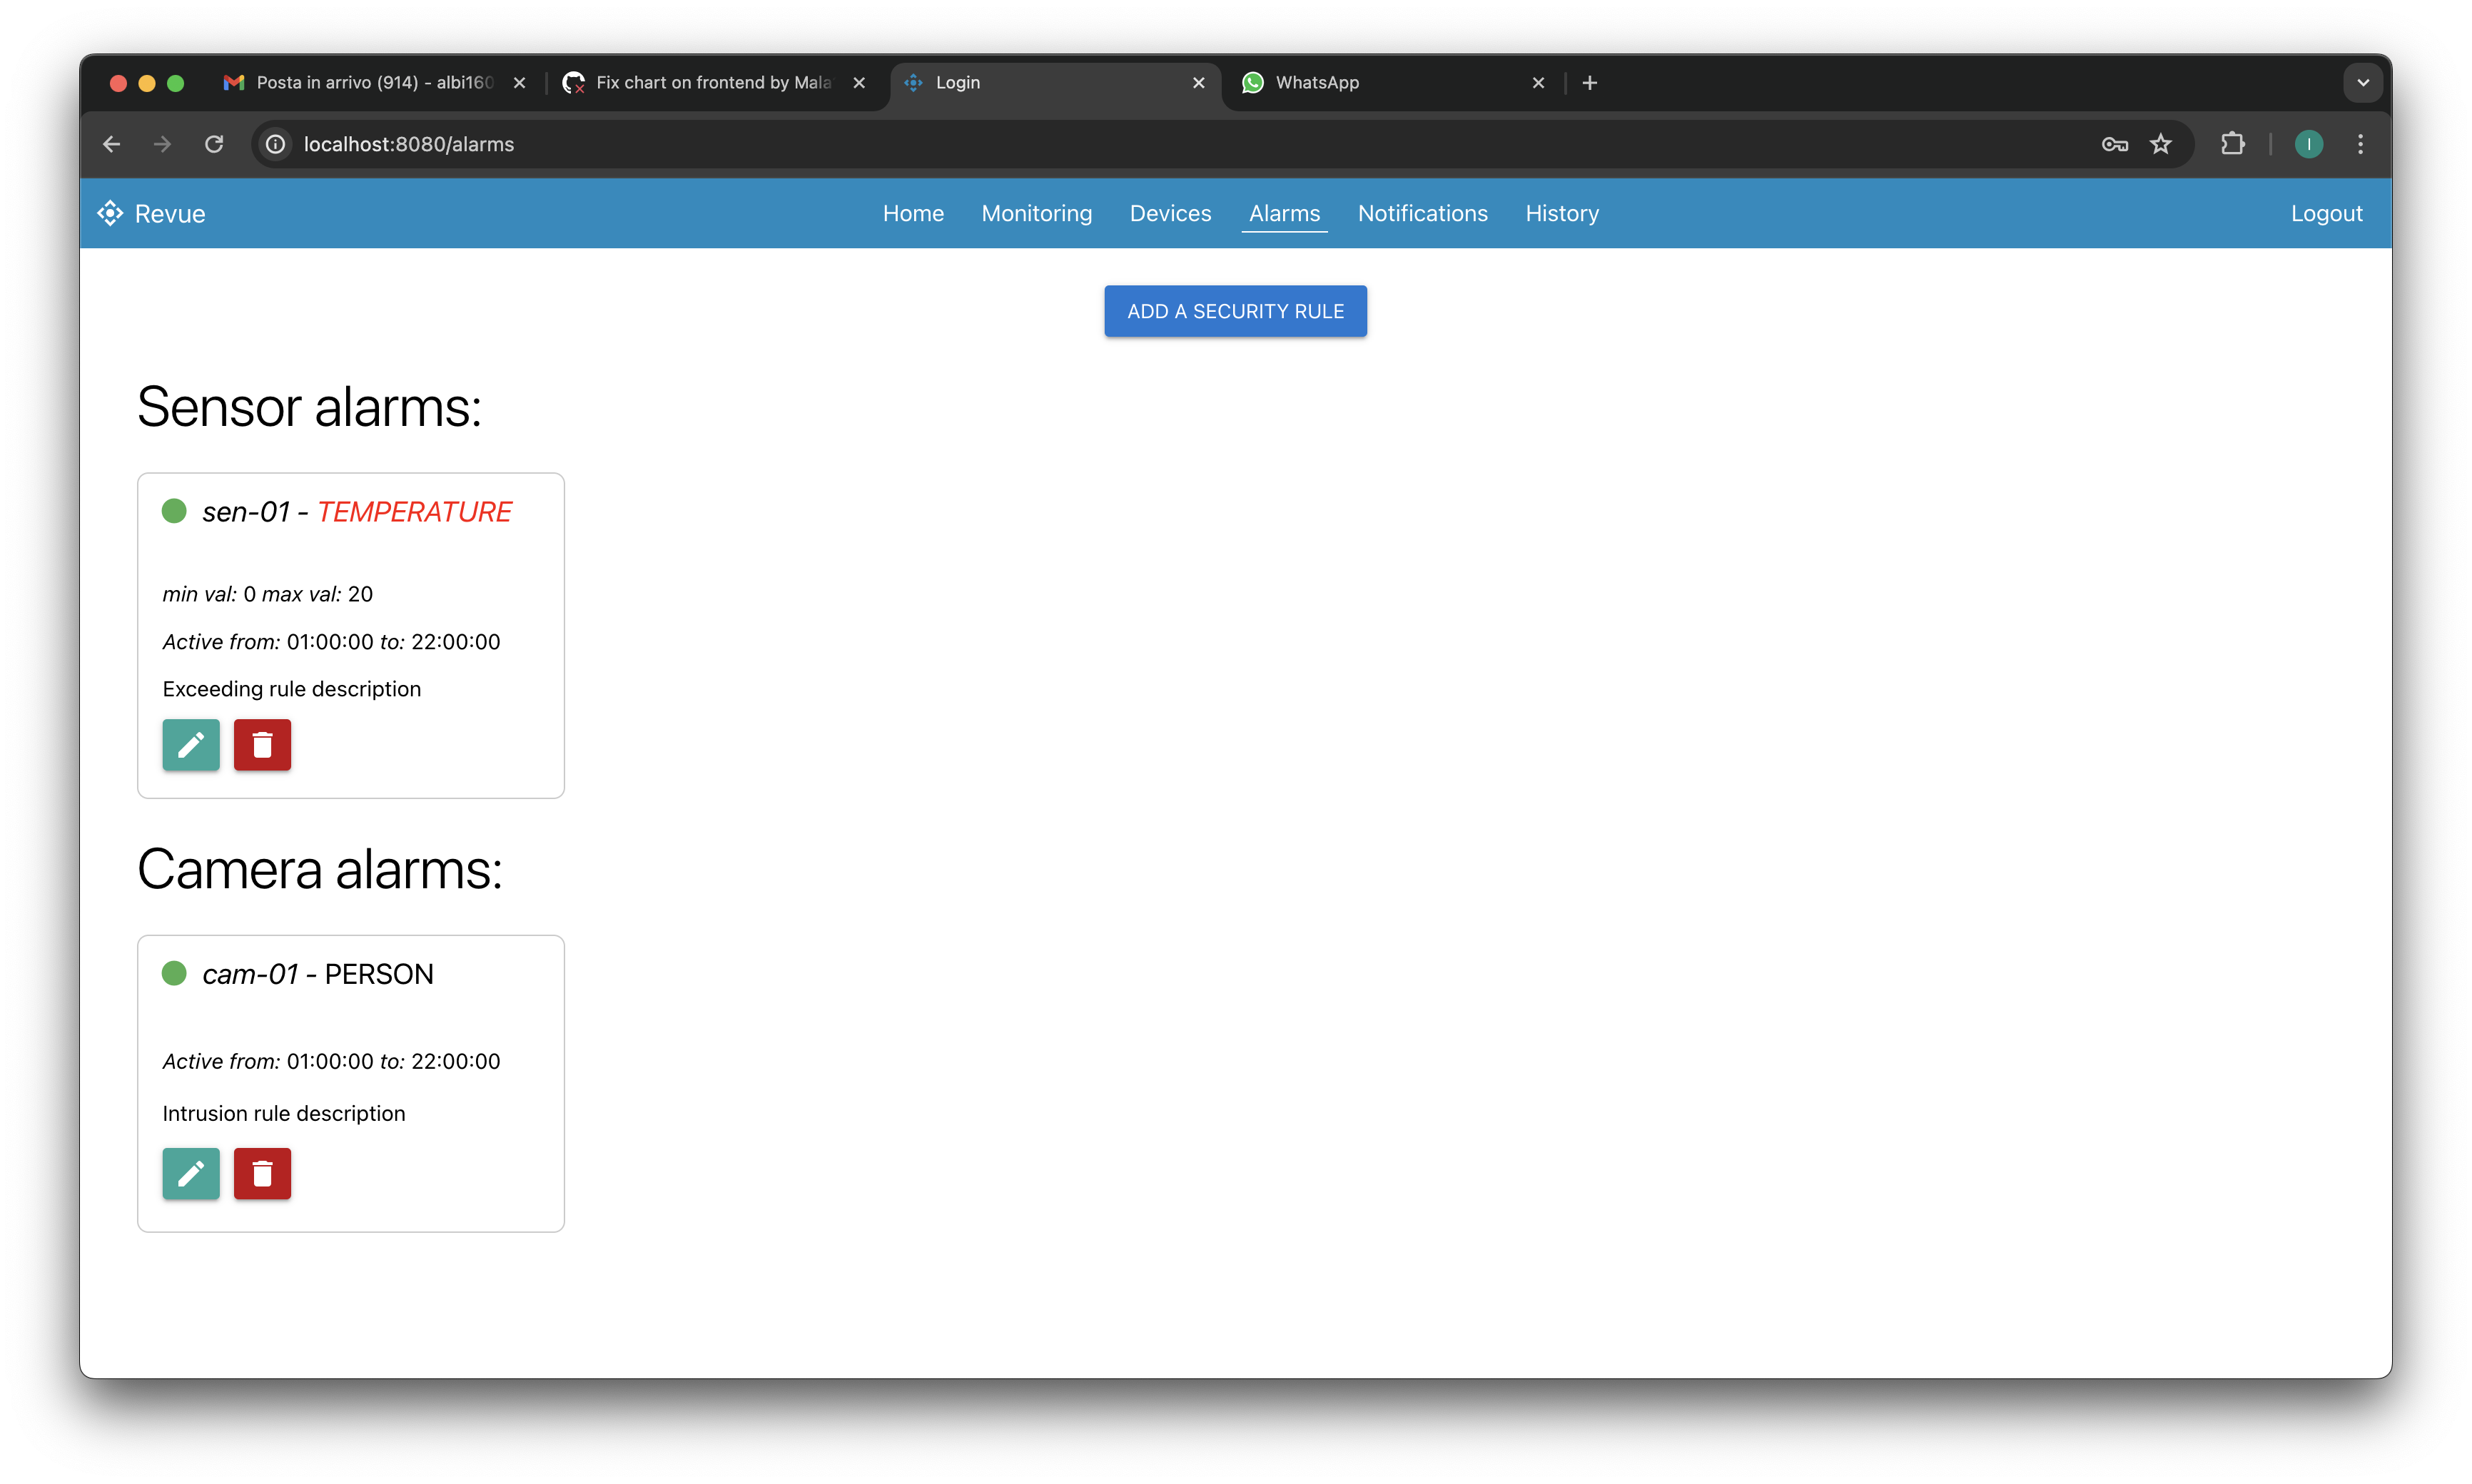
\includegraphics[scale=0.25]{img/usage/security_rule_view}
        \caption{Security rule view}
        \label{fig:security-rule-view}
    \end{figure}

    Both usages of the system consent to the user to add, delete or modify a device or a security rule configuration.

    \begin{figure}
        \centering
        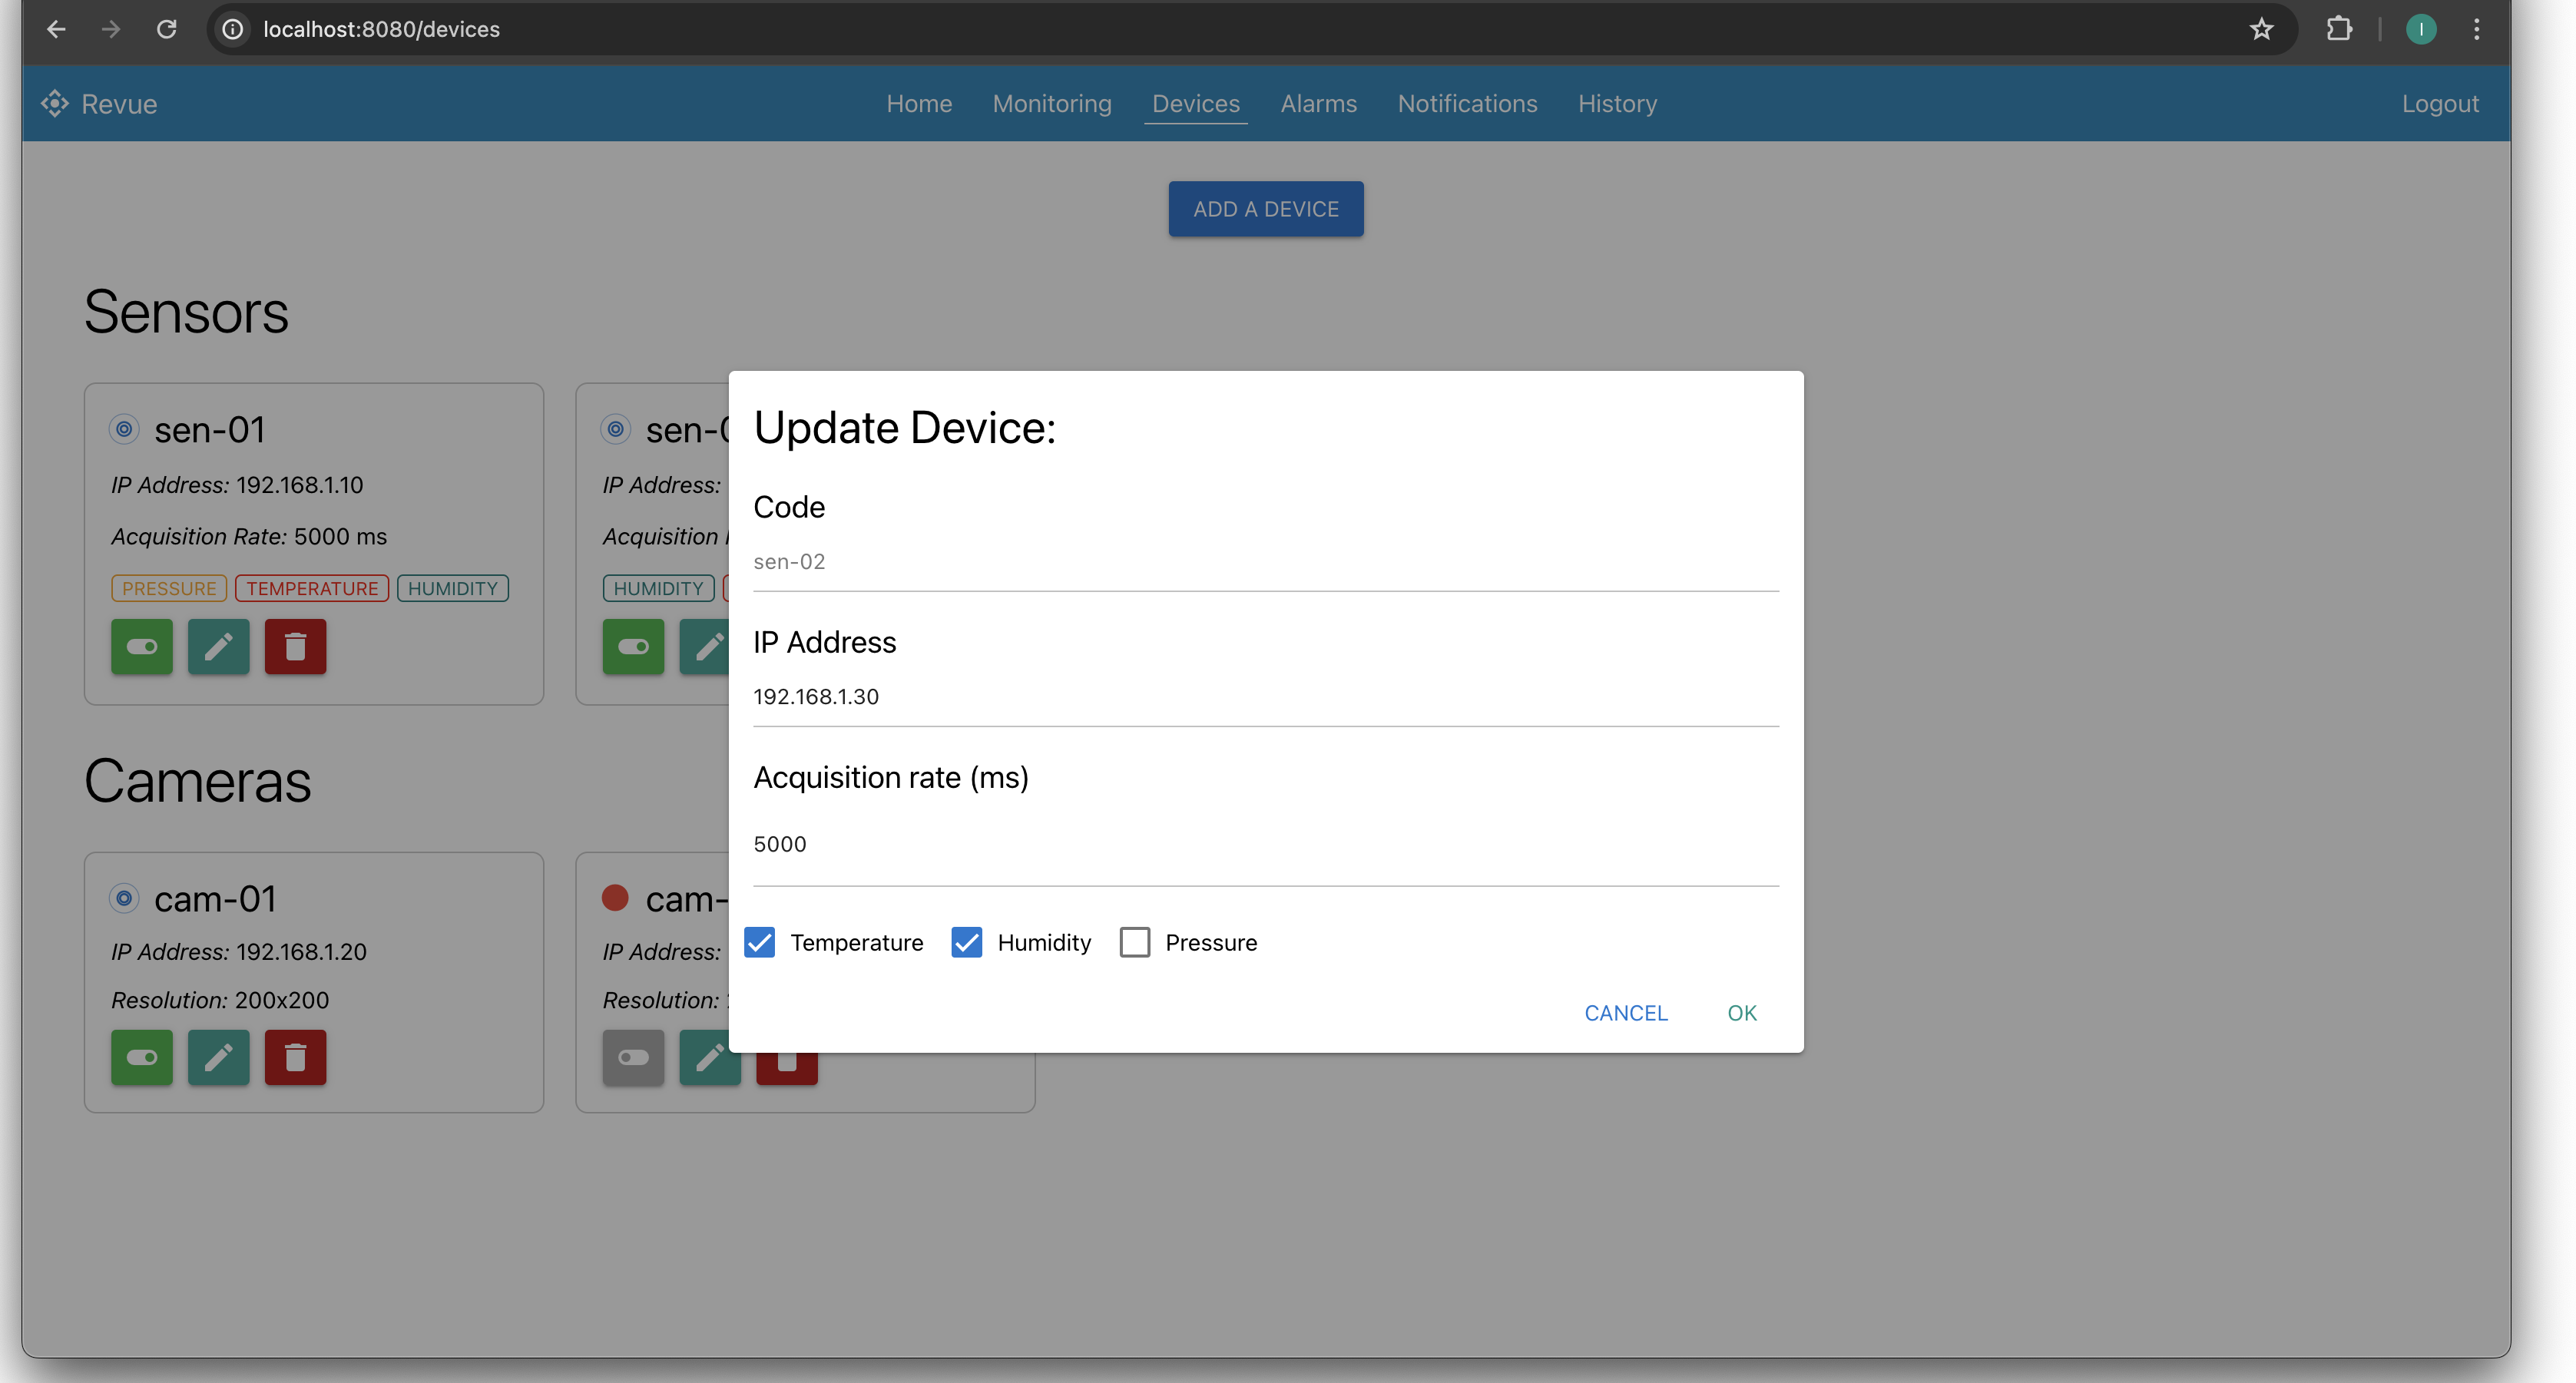
\includegraphics[scale=0.25]{img/usage/update_device_view}
        \caption{Updating a device}
        \label{fig:update-device-view}
    \end{figure}
    \begin{figure}
        \centering
        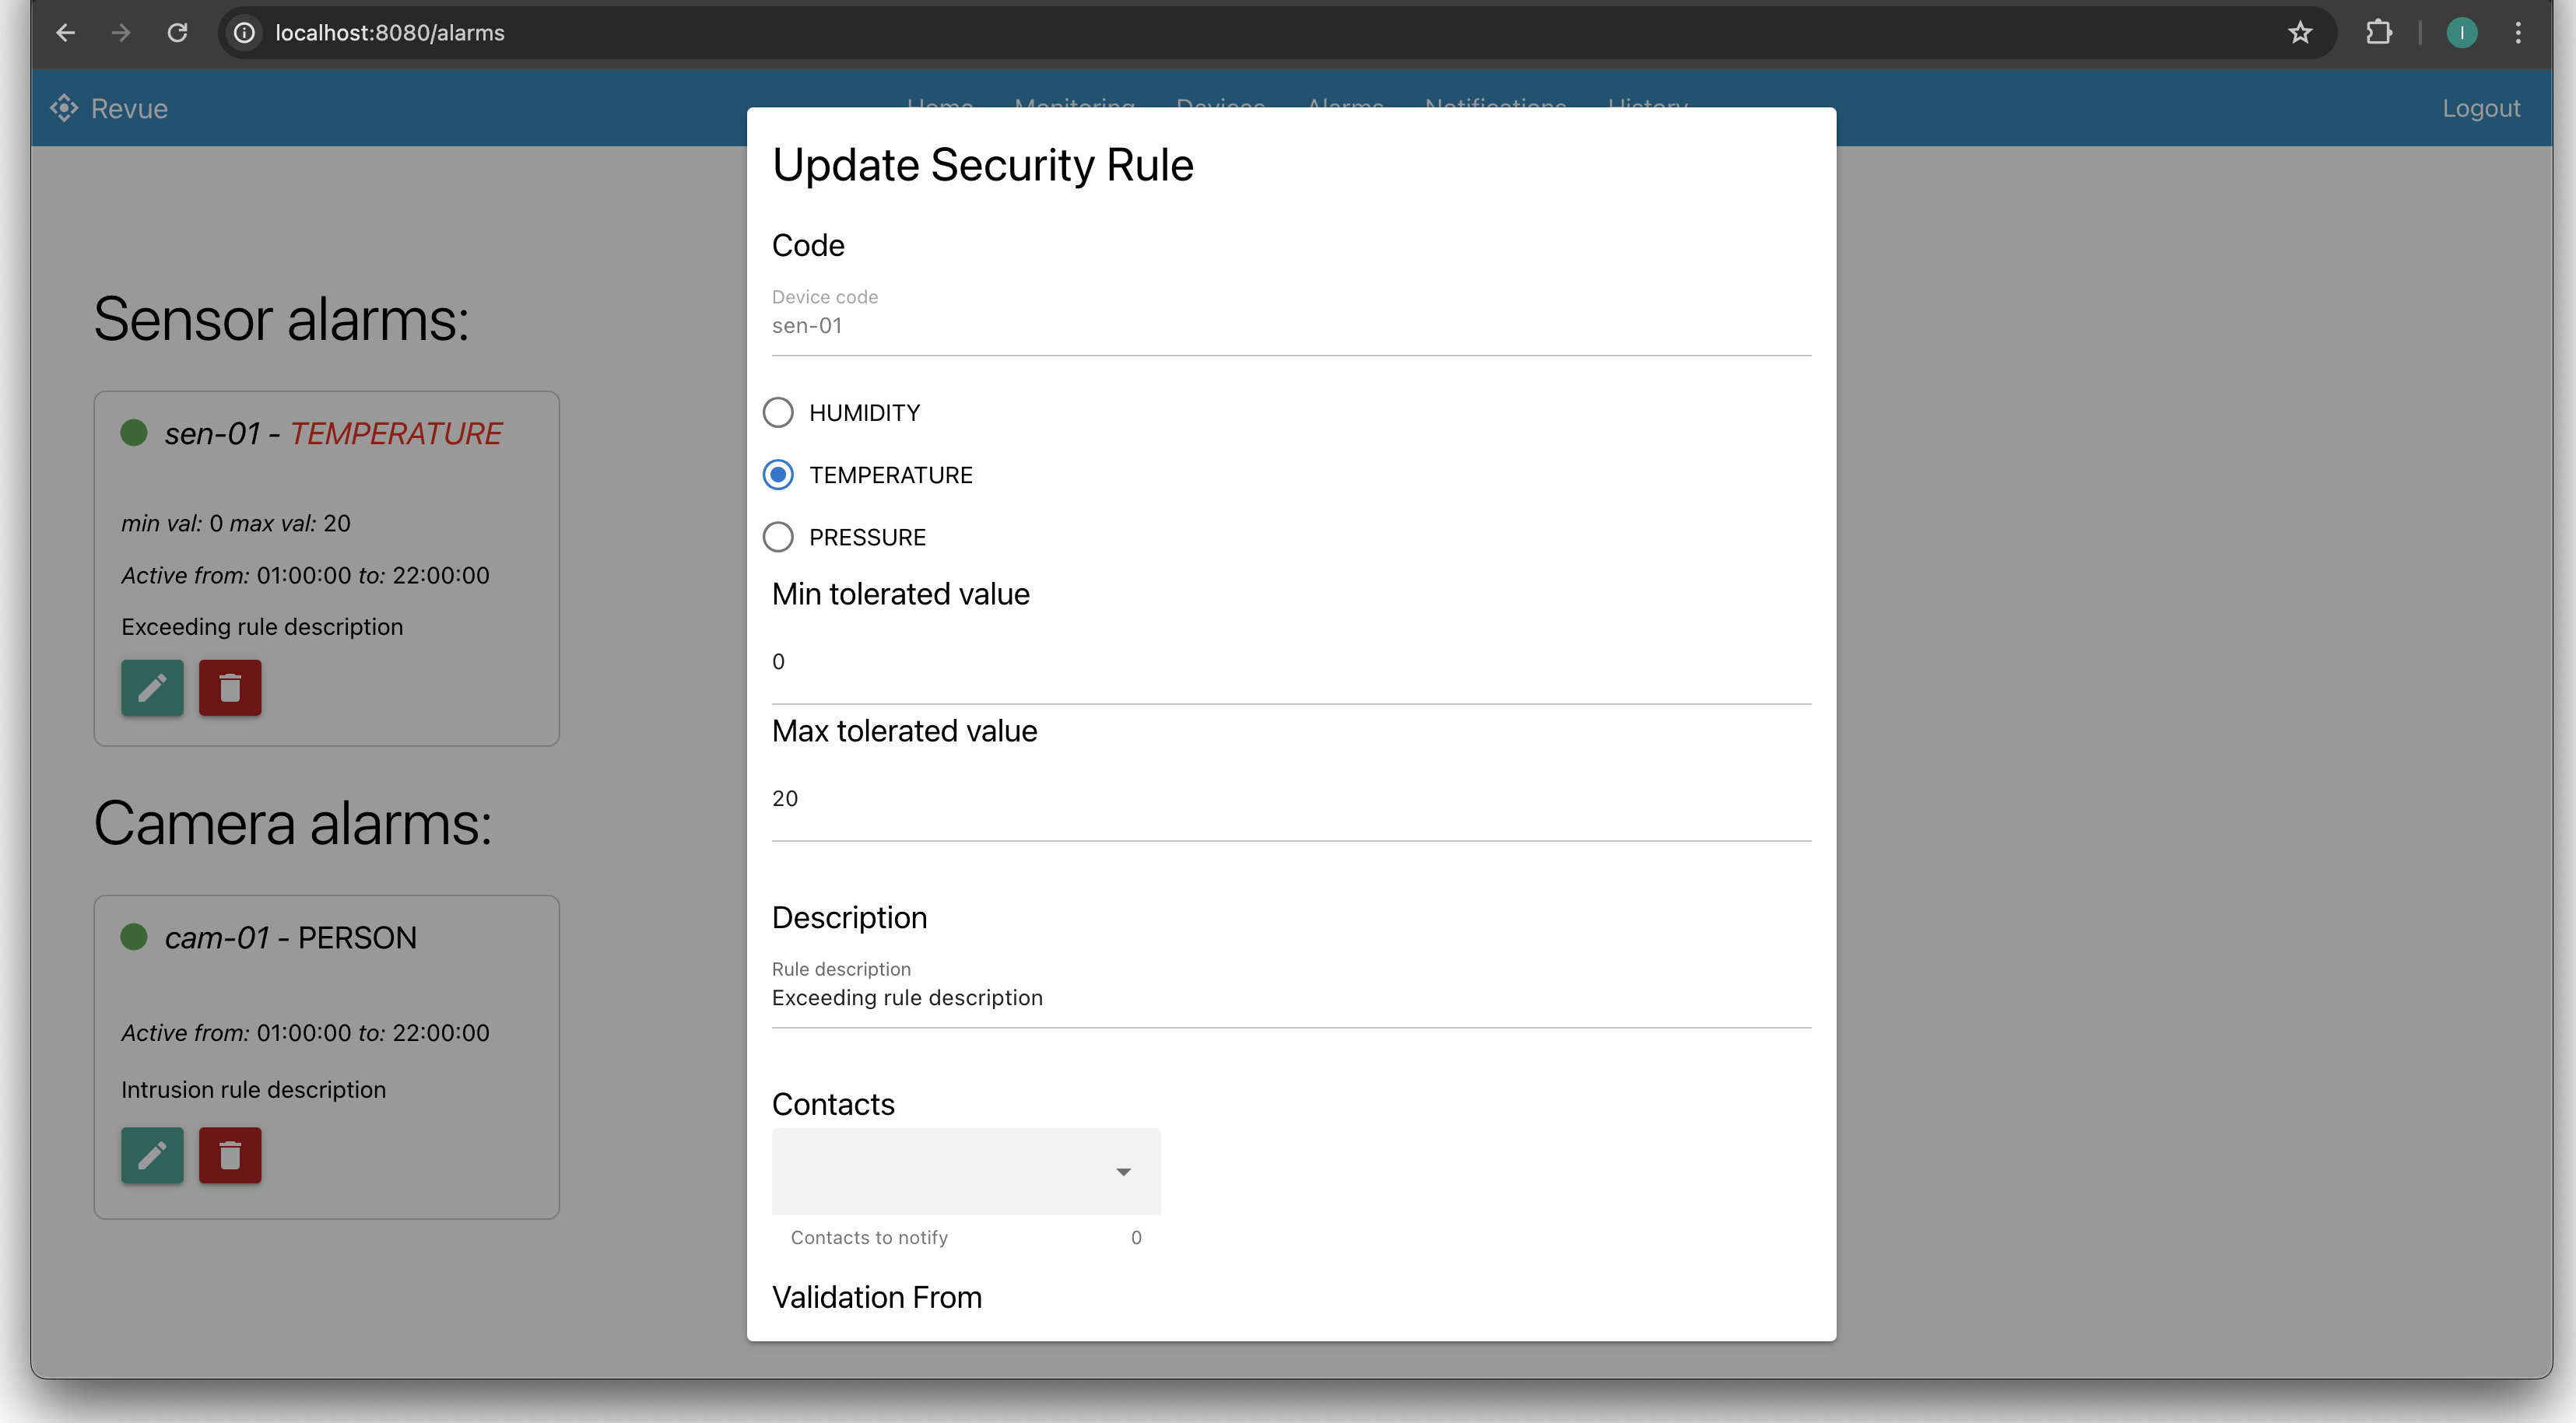
\includegraphics[scale=0.25]{img/usage/update_security_rule_view}
        \caption{Updating a security rule}
        \label{fig:update-security-rule-view}
    \end{figure}

    Moreover, the user can consult the history of produced data or all the notifications received by the system.

    \begin{figure}
        \centering
        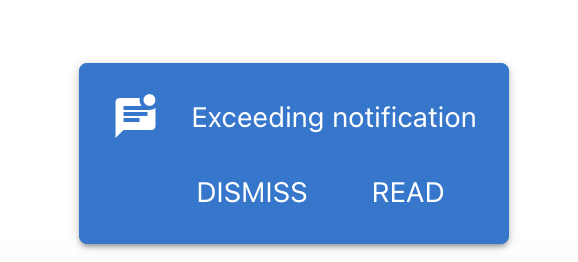
\includegraphics[scale=0.6]{img/usage/notification_example_view}
        \caption{Notification alert}
        \label{fig:notification-example-view}
    \end{figure}
    \begin{figure}
        \centering
        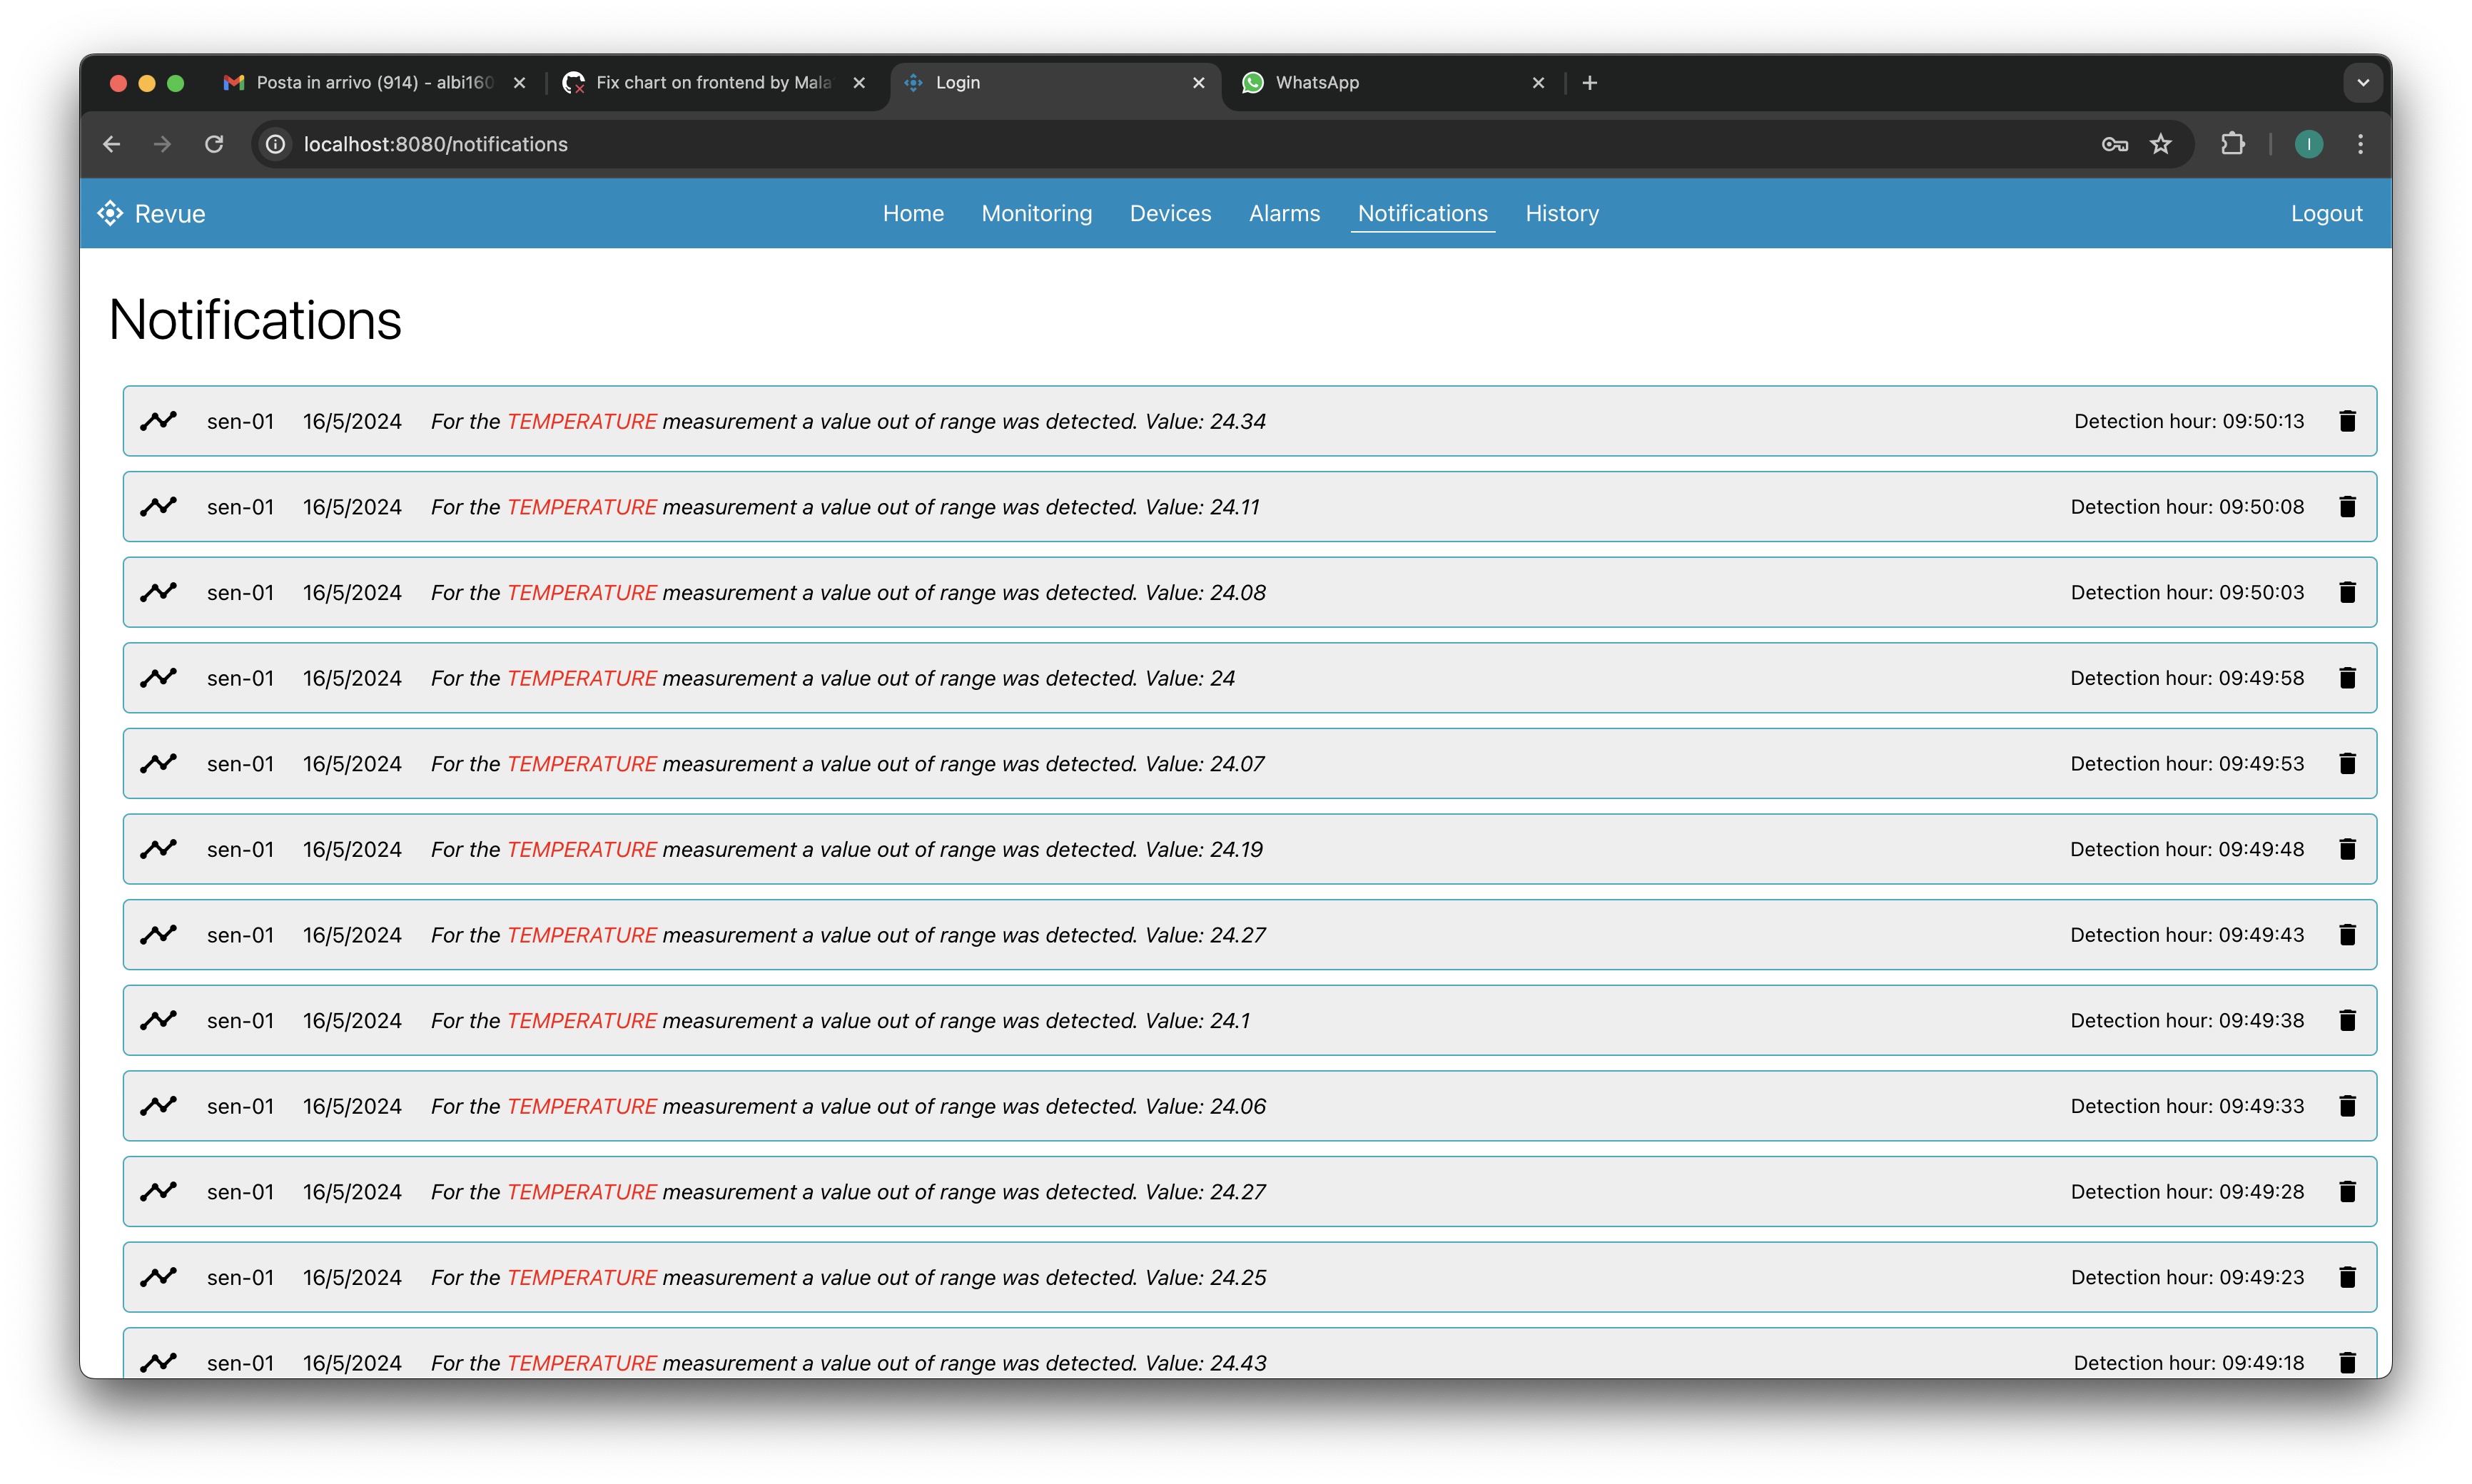
\includegraphics[scale=0.25]{img/usage/notification_view}
        \caption{Security rule view}
        \label{fig:notification-view}
    \end{figure}
    \begin{figure}
        \centering
        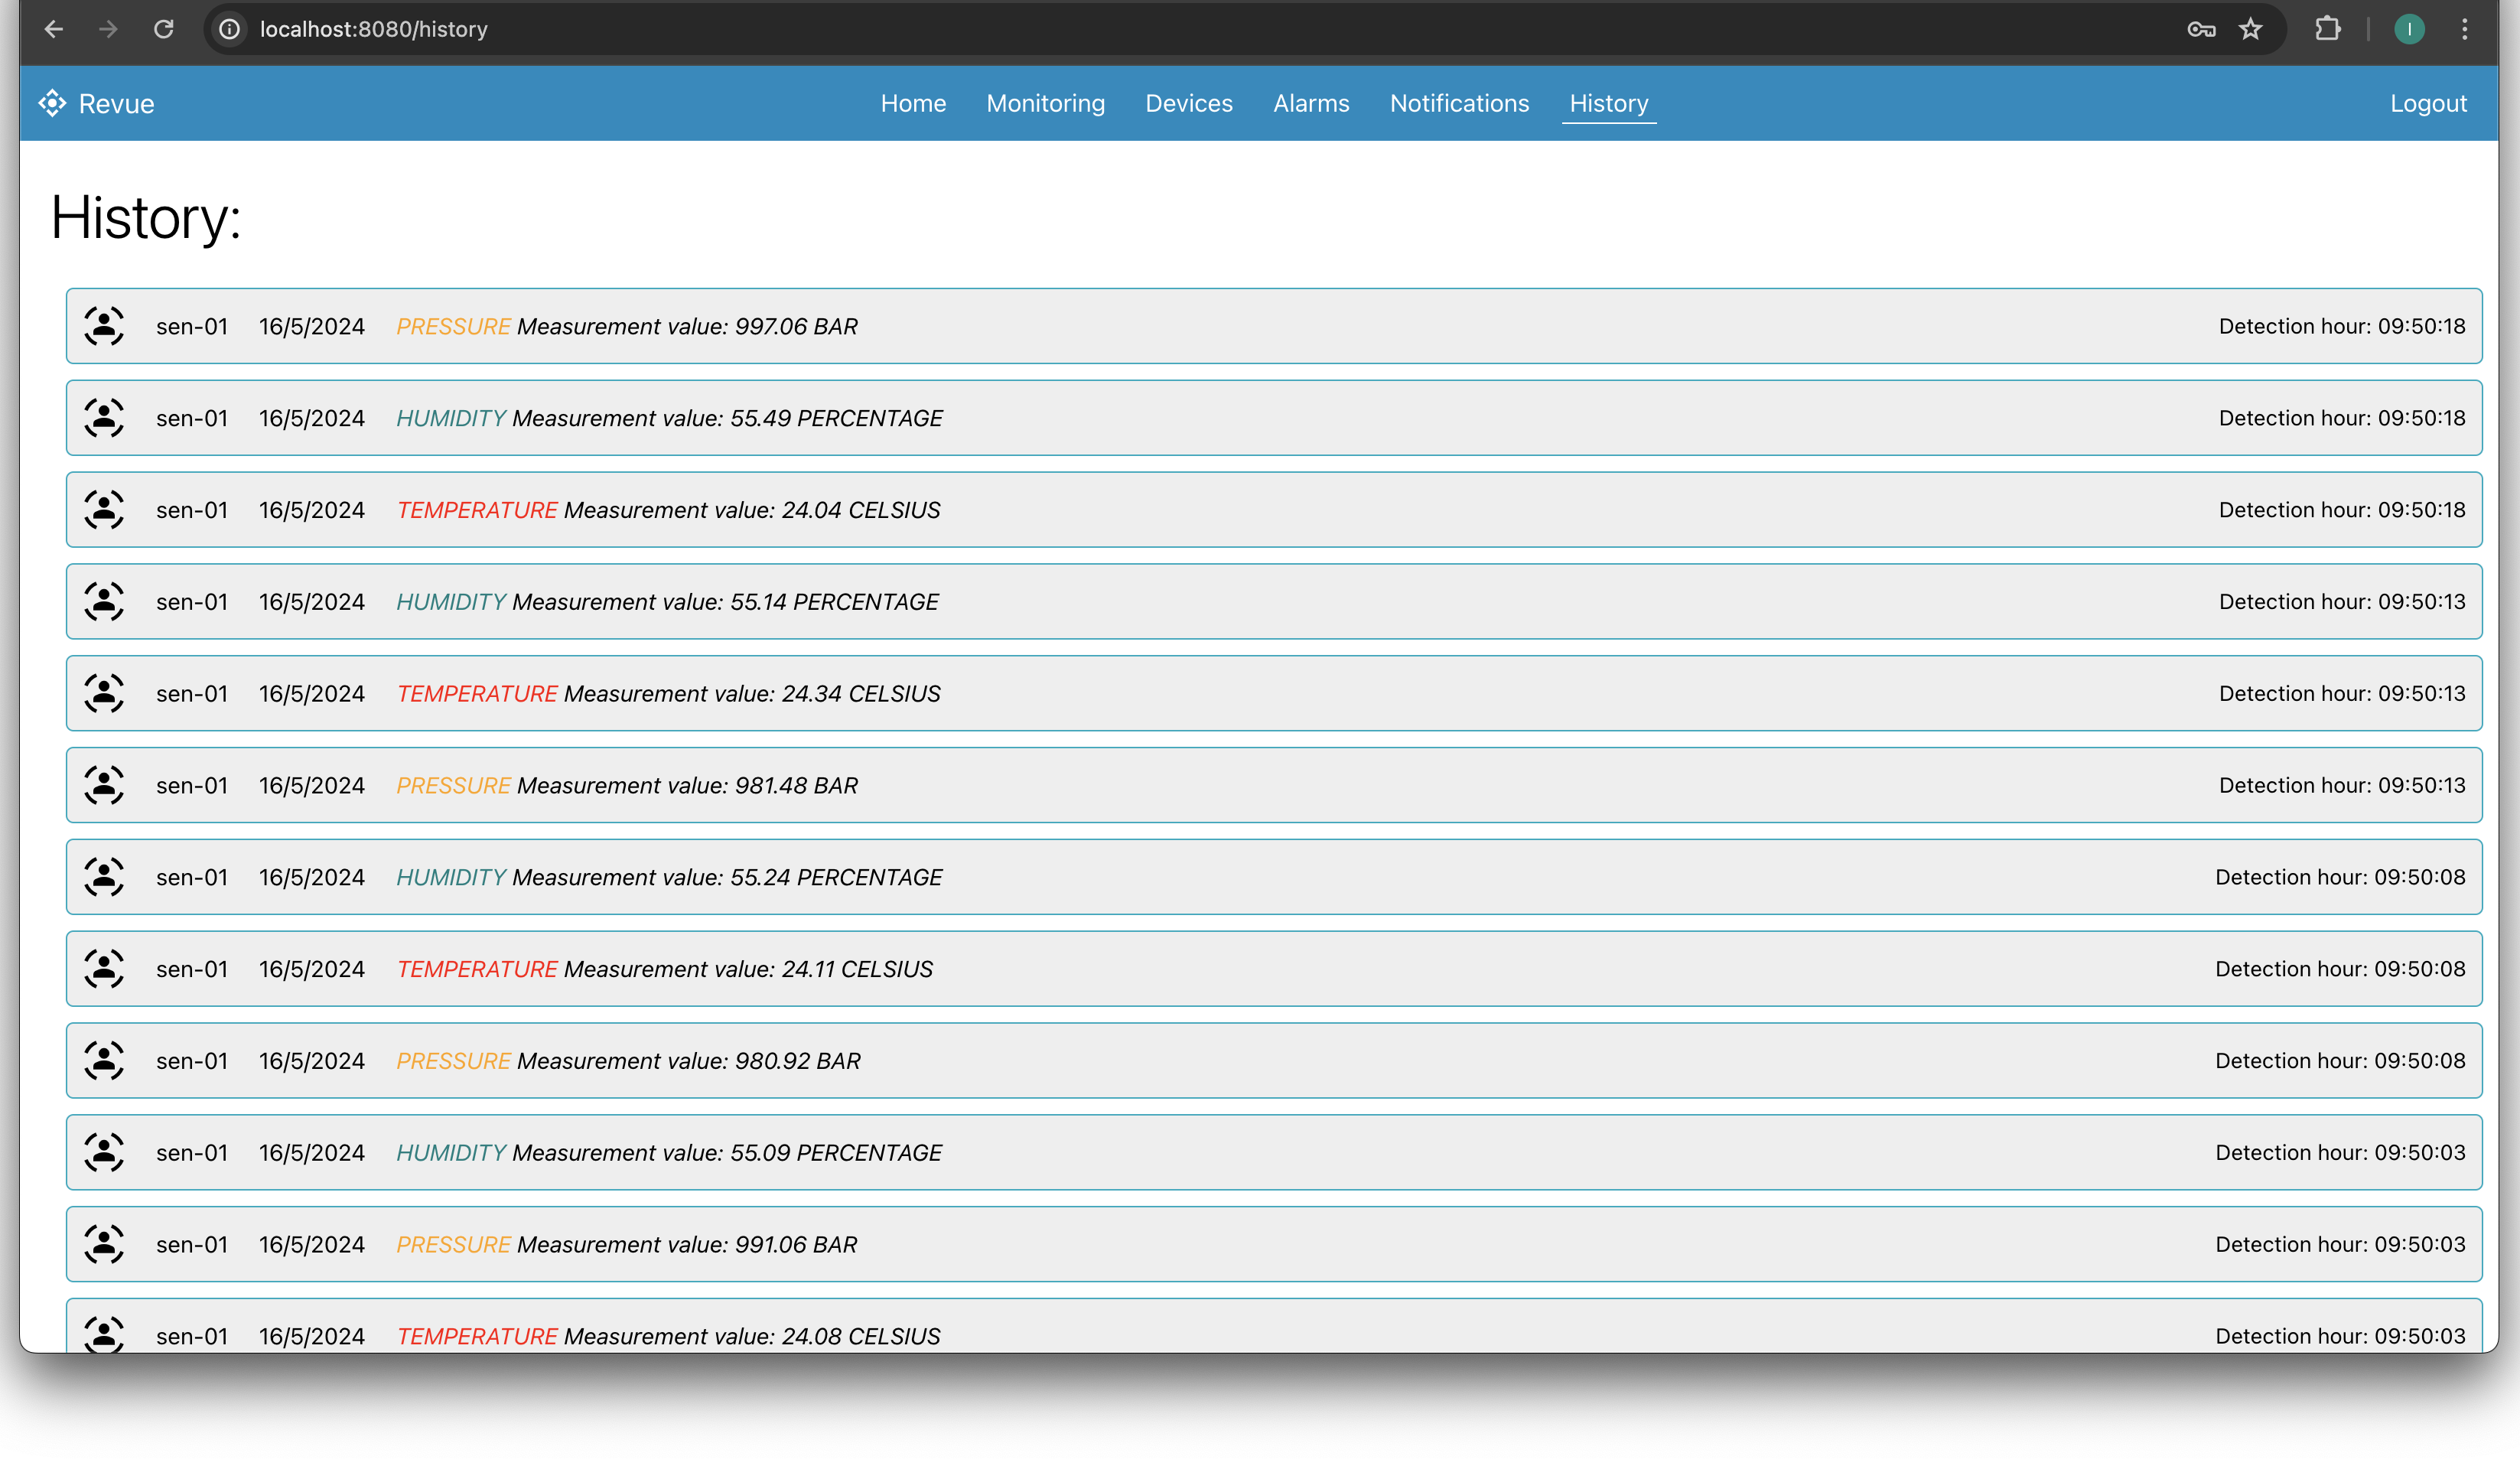
\includegraphics[scale=0.25]{img/usage/log_view}
        \caption{Security rule view}
        \label{fig:log-view}
    \end{figure}


    \section{Conclusions}

    \subsection{Future Works}

    Future developments of this system will certainly have to enrich the user experience to exploit all the possible features offered by the system.
    Certainly a well-designed user section and the introduction of roles could open up to better configurability.

    Real-time video consultation could be improved with the introduction of video recording functions as well as a recorded history,
    which has been put aside for now due to time restrictions.

    Furthermore, Web of Things perspective is the objective for next courses' exams.
    %
    This will lead to the refactor of existent API, the addition of Thing Descriptions, etc.
    %
    Also, an upgrade to the RESTful API could be considered to make them \href{https://en.wikipedia.org/wiki/HATEOAS}{HATEOAS} compliant.

    Another point that could certainly be worked on would be a refinement of the system design to make it even more scalable and maintainable.
    %
    In particular, device management, which is currently part of the monitoring service, surely will be improved with the introduction of a dedicated service.

    For the deployment of the system, the use of Kubernetes (in particulare k3s) will be considered to manage the containers in a more efficient way.
    %
    The goal is to deploy the system in a Raspberry PI cluster.

    \subsection{What did we learned}

    This project allowed us to deepen our knowledge of the microservices architecture and to understand the advantages and disadvantages of this approach.

    Moreover, it helped us to experiment with new technologies such as Kafka, and more in-depth testing.

    Fault tolerance testing has been particularly interesting and has allowed us to understand how to manage the system in case of failure of one or more services, validating the reliability of the system.

%    \nocite{*} % Includes all references from the `references.bib` file
%    \bliographystyle{plain}
%    \bibliography{references}

\end{document}
